\documentclass[preprint,12pt,a4paper]{elsarticle}

\usepackage[utf8]{inputenc}
\usepackage[margin=2cm]{geometry}
\usepackage{amsmath,amssymb,amsfonts}
\usepackage{booktabs}
\usepackage{tabularx}
\usepackage{multirow}
\usepackage{siunitx}
\sisetup{
  uncertainty-mode = separate,
  mode = match,
  propagate-math-font = true,
  reset-math-version = false,
  reset-text-family = false,
  reset-text-series = false,
  reset-text-shape = false,
  text-family-to-math = true,
  text-series-to-math = true,
  retain-explicit-plus = true,
  range-units = single,
  list-units = single
}
\DeclareSIUnit\kWh{kWh}
\DeclareSIUnit\MWh{MWh}
\DeclareSIUnit\kUSD{kUSD}
\DeclareSIUnit\USD{USD}
\DeclareSIUnit\tCOtwoe{tCO_{2}e}
\DeclareSIUnit\gCOtwoe{gCO_{2}e}
\DeclareSIUnit\kgCOtwoe{kgCO_{2}e}
\DeclareSIUnit\pp{pp}
\DeclareSIUnit\XAF{XAF}
\DeclareSIUnit\yr{yr}
\DeclareSIUnit\ppm{ppm}
\usepackage{physics}
\AtBeginDocument{\RenewCommandCopy\qty\SI}
\usepackage[version=4]{mhchem}
\usepackage{graphicx}
\graphicspath{{figures/}}
\usepackage{xcolor}
\usepackage{xr}
\usepackage{lineno}
\usepackage[hidelinks]{hyperref}
\usepackage[capitalise,noabbrev]{cleveref}

\externaldocument[sm:][nocite]{RE_SM_2611}

\journal{Renewable Energy}

\begin{document}

\begin{frontmatter}

\title{Scale-Bridging Techno-Economic, Microclimatic, and Open-Quantum Assessment of Semi-Transparent Organic Agrivoltaics for Sub-Saharan Perennial Crops}

\author[udla]{Steve Cabrel Teguia Kouam}
\author[uy1]{Theodore Goumai Vedekoi}
\author[uy1]{Jean-Pierre Tchapet Njafa}
\author[udla]{Jean-Pierre Nguenang}
\author[uy1]{Serge Guy Nana Engo\corref{cor1}}
\ead{serge.nana-engo@facsciences-uy1.cm}

\cortext[cor1]{Corresponding author.}
\address[udla]{Department of Physics, Faculty of Science, University of Douala, P.O. Box 24157, Douala, Cameroon}
\address[uy1]{Department of Physics, Faculty of Science, University of Yaound\'e~I, P.O. Box 812, Yaound\'e, Cameroon}

\begin{abstract}
Semi-transparent organic photovoltaics (ST-OPVs) are promoted for tropical agrivoltaics assuming spectral filtering cools crops without silicon's light penalty and modulates photosynthetic quantum coherence. We test both premises via a matched-shade counterfactual model across Cameroon's Arabica coffee, Penja white pepper, and highland tea chains, coupling PM6:Y6 transfer-matrix optics, \qty{8760}{\hour} ERA5--FvCB--FAO-56 physiology, battery dispatch, replacement-aware LCA, and $N=\num{10000}$ Saltelli--Sobol draws alongside steady-state bounds on three 14-site LHCII Hamiltonians. Shapley attribution exposes a seasonal inversion: dry-season cooling lifts yields (\qtyrange{8.8}{30.2}{\percent}), whereas monsoon light deficits turn annual yields negative in coffee (\qty{-7.08}{\percent}) and tea (\qty{-3.35}{\percent}) at \qty{40.6}{\percent} shade, leaving rainfed pepper positive (\qtyrange{+7.43}{+8.16}{\percent}). At matched shade, ST-OPV and c-Si crop yields differ by $\le \num{1.1}$~percentage points and spectral selectivity adds \qtyrange{-0.2}{-0.7}{\percent}: shade fraction governs response. Tea storage lifts solar fraction to \qty{99.9}{\percent}. Dual Sobol analysis separates bankability (tariffs and WACC govern $\mathrm{NPV}_{\mathrm{OPV}}$) from technology choice: baseline ST-OPV (\qty{35}{\USD\per\square\meter}, $T_{80}=\qty{5}{\yr}$) trails c-Si NPV in \qtyrange{77}{89}{\percent} of draws (\qtyrange{75}{88}{\percent} at zero carbon). Carbon parity needs $T_{80}\ge \qtyrange{7.4}{8.1}{\yr}$, while economic parity (pepper only) needs \qty{15}{\USD\per\square\meter} modules with $T_{80}\ge \qty{16.3}{\yr}$. Quantum shifts stay $\le \num{3.4e-5}$ ($\le \num{2.1e-3}$ HEOM envelope, $S_{Ti}\le \num{2.6e-7}$). Module cost, stability, and shade timing govern deployment.
\end{abstract}

\begin{keyword}
PM6:Y6 transfer-matrix optics \sep Cameroon highlands \sep Penja white pepper \sep Seasonal regime inversion \sep Environmental carbon payback \sep Sobol global sensitivity
\end{keyword}

\end{frontmatter}
\linenumbers

% ==============================================================================
\section{Introduction}
\label{sec:intro}
% ==============================================================================

Dual land-use intensification via agrivoltaic (AV) co-production offers a concrete pathway to pair rural clean electrification and agricultural modernization with climate adaptation for heat-stressed perennial crops~\cite{Dupraz2011,Valle2017,Weselek2019,BarronGafford2019,FAO2022,Asaa2024,Campana2025,Mahim2025}. Across Sub-Saharan Africa and humid--dry tropical highlands worldwide, high-value perennial cash crops---such as highland Arabica coffee, specialty spices, and orthodox tea---sustain smallholder cooperatives exposed both to intensifying dry-season vapor pressure deficits (VPD) and to unreliable, diesel-backed post-harvest processing grids. Unlike temperate annuals or arid-zone row crops, however, tropical highland perennials face a seasonal optical dilemma: extreme dry-season radiative heat (\qtyrange{2.8}{4.9}{\kilo\pascal} VPD) invites canopy shading, whereas persistent wet-season monsoon cloudiness (\numrange{0.42}{0.50} diffuse sky fraction) risks light starvation under year-round structures. Conventional elevated opaque crystalline silicon (c-Si) arrays deliver low levelized cost of electricity (LCOE)~\cite{Amaducci2018,TemizDincer2024,Zidane2025}, yet require heavy galvanized steel substructures for farm clearance ($\ge\qty{3.5}{\meter}$) and cast spectrally neutral shadows that alter soil moisture, microclimate telemetry, and monsoon-season photosynthesis~\cite{Marrou2013,Elamri2018,MaLu2022,Wu2023Energies,Bellone2024,Zainali2025,DiDomenico2026}.

Semi-transparent organic photovoltaics (ST-OPVs) based on narrow-bandgap non-fullerene acceptors (NFAs) such as Y6 blended with wide-bandgap polymer donors such as PM6~\cite{Lunt2011,Yuan2019,Cui2019,Liu2020,Cui2021,Shen2025NatCommun} have been advocated as spectrally tailored AV canopies~\cite{Ravishankar2020,Thompson2020}. By absorbing ultraviolet and near-infrared photons (\qtyrange{700}{950}{\nano\meter}) while transmitting photosynthetically active radiation (PAR, \qtyrange{400}{700}{\nano\meter}) on lightweight tensile structures, ST-OPVs in principle mitigate PAR competition while lowering structural balance-of-system (BOS) steel requirements~\cite{Machui2014,Ravilla2024}. Simultaneously, comparison between photosynthetic and photovoltaic conversion efficiencies~\cite{Blankenship2011} and ultrafast spectroscopic evidence of transient coherence in photosynthetic light-harvesting complex II (LHCII)~\cite{Collini2010,Novoderezhkin2011,Huelga2013,Fleming2015,Scholes2015,Cao2020,TeguiaKouam2026} have prompted speculation on whether spectrally filtered canopies alter primary excitonic energy transfer (EET) efficiency~\cite{Kassal2013,Kim2025SciAdv}.

A critical synthesis of existing literature (\cref{tab:lit_matrix}) reveals three cross-scale methodological gaps that prevent rigorous engineering and policy decisions for tropical ST-OPVs. First, seasonal regime inversion has rarely been quantified against matched-shade opaque counterfactuals. Most process-based agrivoltaic models focus on temperate or dry summer annuals~\cite{Dupraz2011,Amaducci2018,Elamri2018,MaLu2022}, whereas greenhouse ST-OPV demonstrations~\cite{Ravishankar2020,Thompson2020} emphasize controlled transmittance without hourly tropical water--energy coupling. Resolving whether fixed shading yields a net annual benefit or penalty across humid--dry perennials---and isolating spectral selectivity from total shade fraction---requires hourly coupling of leaf energy balance, Farquhar--von Caemmerer--Berry (FvCB) photosynthetic kinetics, photoinhibition relief, and FAO-56 root-zone water conservation evaluated directly against both traditional agroforestry ($S_1$) and elevated c-Si at equal shade~\cite{Farquhar1980,Medlyn2011,Elamri2018,Adeh2019,MaLu2022}.

\begin{table}[htbp]
  \centering
  \caption{Methodological positioning of the present scale-bridging assessment relative to established agrivoltaic, semi-transparent OPV, techno-economic, and open-quantum literature streams.}
  \label{tab:lit_matrix}
  \scriptsize
  \renewcommand{\arraystretch}{1.15}
  \resizebox{\textwidth}{!}{
  \begin{tabular}{@{}*{6}{>{\raggedright\arraybackslash}p{2.75cm}}@{}}
    \toprule
    \textbf{Literature stream} & \textbf{Climate / crop scope} & \textbf{Optical canopy model} & \textbf{Dispatch, TEA \& LCA} & \textbf{Quantum dynamics} & \textbf{Primary scope \& gap} \\
    \midrule
    Opaque elevated AV modeling~\cite{Dupraz2011,Amaducci2018,Elamri2018,MaLu2022,Zainali2025} & Temperate / arid annuals \& perennials & Opaque neutral shade projection & Agronomic yield \& LER; limited BESS/LCA & None & Establishes crop water--light mechanics; omits NFA spectral optics \\
    ST-OPV greenhouses \& crops~\cite{Ravishankar2020,Thompson2020,Shen2025NatCommun} & Controlled greenhouses / lettuce, crops & Wavelength-selective TMM (PM6:Y6) & Thermal energy balance; zero cooperative TEA/LCA & None & Demonstrates spectral selectivity; lacks humid--dry outdoor seasonal testing \\
    AV regional TEA, LCA \& MC~\cite{Ravilla2024,TemizDincer2024,Zidane2025} & Temperate US / Europe / utility grids & Fixed or tilted opaque/bifacial c-Si & Full TEA/LCA or European MC; no tropical dispatch & None & Identifies CAPEX/BOS dominance; excludes tropical OPV replacement \\
    Open-quantum LHCII EET~\cite{BrumerShapiro2012,Kassal2013,Kim2025SciAdv,TeguiaKouam2026} & Molecular pigment complexes & Idealized or unfiltered pumping & None & Pulsed HEOM / MesoHOPS vs.\ CW NESS & Defines quantum--classical physics; uncoupled from farm economics \\
    \textit{Present study} & \textit{Tropical wet--dry perennials (3 crops)} & \textit{Calibrated PM6:Y6 TMM vs.\ matched c-Si} & \textit{Hourly BESS dispatch, dual-FU LCA, $N=\num{10000}$ Sobol} & \textit{3 LHCII Hamiltonians, HEOM/MesoHOPS + NPV} & \textit{Falsifiable counterfactual test across 5 scales} \\
    \bottomrule
  \end{tabular}
  }
\end{table}

Second, module techno-economics, replacement-aware life-cycle assessment (LCA), and cooperative post-harvest dispatch are seldom integrated within a single decision framework~\cite{Ravilla2024,Zidane2025}. Because current organic photovoltaic lifetimes remain finite ($T_{80} = \qtyrange{5}{10}{\yr}$)~\cite{Machui2014,Gambhir2016,Wang2023,Ravilla2024}, periodic module replacement elevates embodied carbon per functional kilowatt-hour while eroding cumulative cash flow. These penalties must be weighed jointly against site-specific processing demand profiles---such as daytime spice drying versus continuous \qty{24}{\hour} tea withering requiring battery energy storage (BESS)---under the zero-subsidy, zero-carbon-price baseline typical of rural agricultural cooperatives, and tested separately for both standalone bankability ($\mathrm{NPV}_{\mathrm{OPV}}$) and technology selection ($\Delta\mathrm{NPV} = \mathrm{NPV}_{\mathrm{OPV}} - \mathrm{NPV}_{\mathrm{Si}}$). Third, the quantum premise behind spectrally tailored canopies remains untested at agricultural system scale. Although 2D electronic spectroscopy and non-Markovian hierarchical equations of motion (HEOM/\allowbreak MesoHOPS) demonstrate fs--ps coherent dynamics under pulsed excitation~\cite{Tanimura1989,Ishizaki2009,Suess2015,Varvelo2021,Lambert2023,Citty2024,TeguiaKouam2026}, prompting hypotheses that spectral filtering could alter excitonic energy transfer~\cite{Kassal2013,Kim2025SciAdv}, natural continuous-wave (CW) sunlight drives incoherent absorption into a non-equilibrium steady state (NESS)~\cite{BrumerShapiro2012,Kassal2013}. Propagating a multi-Hamiltonian CW steady-state bound through crop assimilation into farm net present value (NPV) tests whether ST-OPV canopy design requires quantum-efficiency objectives or can rely exclusively on classical radiometric metrics.

To resolve these coupled physical and economic trade-offs, this study addresses two central questions across western Cameroon's three flagship perennial chains---Arabica coffee (\textit{Coffea arabica}, Foumbot), Protected Geographical Indication (PGI) Penja white pepper (\textit{Piper nigrum}~L., Njombe-Penja), and highland tea (\textit{Camellia sinensis}, Djuttitsa)---whose VPD, diffuse cloudiness, and processing load regimes span archetypal wet--dry tropical highlands: (i) what dynamic balance of leaf cooling, VPD conservation, monsoon PAR loss, and bounded spectral or quantum redistribution governs rainfed crop yields; and (ii) under hourly tropical seasonality, cooperative processing loads, and zero-subsidy baseline economics, how do PM6:Y6 ST-OPV and elevated opaque c-Si compare in crop yield relative to open sun, land equivalent ratio (LER), 20-year array NPV per installed hectare, and life-cycle carbon intensity, and how do these outcomes vary with crop, dispatch, module cost, and stability? Furthermore, when bounded across three independent LHCII Hamiltonians under incoherent solar illumination, does filtered excitonic coherence contribute materially to modeled agronomic yield or financial return? By separating shade from spectral effects through Shapley attribution, coupling replacement-aware LCA with Dual Sobol parity frontiers, and propagating a deliberately conservative quantum lever through the same modeling chain, this work evaluates spectral enhancement and quantum modulation as model-based, testable system-scale hypotheses.

% ==============================================================================
\section*{Nomenclature}
% ==============================================================================
\noindent
{\scriptsize
  \resizebox{\textwidth}{!}{
  \begin{tabular}{@{}ll@{\hspace{1.2cm}}ll@{}}
    \toprule
    \textbf{Symbol / Acronym} & \textbf{Definition (Units)} & \textbf{Symbol / Acronym} & \textbf{Definition (Units)} \\
    \midrule
    $\mathrm{APT}$ & Average photosynthetic transmittance (\qtyrange{400}{700}{\nano\meter}, \unit{\percent}) & $S_{i}, S_{Ti}$ & First-order and total-order Sobol indices (--) \\
    $\mathrm{AWC}$ & Root-zone available water capacity (\unit{\milli\meter}) & $T_{80}$ & Time to \qty{80}{\percent} initial PV PCE (\unit{\yr}) \\
    $\mathrm{BESS}$ & Battery energy storage system (LFP, \unit{\kWh}) & $T_{\mathrm{leaf}}, T_{\mathrm{PV}}$ & Leaf and PV module temperatures (\unit{\celsius}) \\
    $\mathrm{BOS}$ & Balance-of-system structural \& electrical cost (\unit{\USD\per\square\meter}) & $T_{\mathrm{OPV}}^{\mathrm{beam}}, T_{\mathrm{OPV}}^{\mathrm{diff}}$ & Normal beam and diffuse transmittance (--) \\
    $C_{\mathrm{mod}}^{\mathrm{OPV}}, C_{\mathrm{BOS}}^{\mathrm{c\text{-}Si}}$ & OPV module and c-Si BOS unit costs (\unit{\USD\per\square\meter}) & $V_{c\max 25}, J_{\max 25}$ & Max carboxylation and electron transport rates (\unit{\micro\mole\per\square\meter\per\second}) \\
    $\mathrm{CW}$ / $\mathrm{NESS}$ & Continuous-wave / non-equilibrium steady state & $\mathrm{VPD}_{95}$ & 95th-percentile dry-season vapor pressure deficit (\unit{\kilo\pascal}) \\
    $\mathrm{ePAR}$ & Extended PAR (\qtyrange{400}{750}{\nano\meter}) & $\mathrm{WUE}$ & Crop water-use efficiency (\unit{\kilogram\per\cubic\meter}) \\
    $F_{\mathrm{lp}}, F_{\mathrm{sky}}$ & Low-PPFD hour fraction and sky view factor (--) & $\Delta\eta_{\mathrm{NESS}}$ & Coherent vs.\ Pauli EET efficiency shift (--) \\
    $\mathrm{GCR}$ & Array ground coverage ratio (--) & $\Delta T_{\mathrm{leaf}}, \Delta Y$ & Leaf cooling (\unit{\celsius}) and crop yield anomaly (\unit{\percent}) \\
    $I_{\mathrm{PI}}, I_{\mathrm{sat}}$ & Photoinhibition and saturation PPFD (\unit{\micro\mole\per\square\meter\per\second}) & $\lambda_D, \gamma_D$ & Drude--Lorentz bath reorganization and cutoff (\unit{\per\centi\meter}) \\
    $k_{\mathrm{RC}}, k_{\mathrm{NPQ}}$ & Reaction-center trapping (\unit{\per\pico\second}) and NPQ rate (\unit{\per\nano\second}) & $\phi_{\mathrm{PAR/PI}}, \phi_{\mathrm{therm}}$ & Shapley PAR and thermal yield contributions (\unit{\percent}) \\
    $\mathrm{LER}, \mathrm{LSF}, \mathrm{LUE}$ & Land equivalent ratio, load solar fraction, light util.\ eff. & $\phi_{\mathrm{VPD/H_2O}}, \phi_{\mathrm{spec+Q}}$ & Shapley water and spectral+quantum contributions (\unit{\percent}) \\
    $\mathrm{NPV}, \mathrm{IRR}, \mathrm{LCOE}$ & Net present value (\unit{\USD\per\hectare}), internal rate of return (\unit{\percent}), LCOE (\unit{\USD\per\kWh}) & $\mathrm{R{:}FR}$ & Red-to-far-red photon flux ratio (--) \\
    \bottomrule
  \end{tabular}
  }
}
\vspace{0.8em}

% ==============================================================================
\section{Materials, site calibration, and scale-bridging methodology}
\label{sec:methods}
% ==============================================================================

All physical, botanical, optical, and economic inputs are consolidated from peer-reviewed physiological datasets and primary regional surveys summarized in Supporting Material~\ref{sm:sec:sm_agro}.

\subsection{Counterfactual design and analytical boundaries}
\label{sec:interpretive}

Because this investigation evaluates a counterfactual engineering problem without paired field agrivoltaic measurements at the three Cameroonian sites, all crop responses represent conditional simulations generated by literature-calibrated process models driven by the full-year 2023 ERA5 reanalysis. Accordingly, conclusions are framed conditionally on model structure and parameter bounds across six counterfactual configurations: an open-field unshaded control ($S_0$), a traditional shade-tree agroforestry reference ($S_1$), elevated opaque crystalline silicon counterfactuals at $\mathrm{GCR}=\qty{40}{\percent}$ and \qty{70}{\percent} ($S_2(\mathrm{c\text{-}Si,\,GCR40})$ and $S_2(\mathrm{c\text{-}Si,\,GCR70})$), baseline PM6:Y6 ST-OPV canopies ($T_{80}=\qty{5}{\yr}$) spanning $\mathrm{APT}=\qtyrange{20}{56}{\percent}$ and $\mathrm{GCR}=\qtyrange{50}{85}{\percent}$ (denoted $S_3(\mathrm{APT}\,x,\,\mathrm{GCR}\,y)$, with the balanced focal design $S_3(\mathrm{APT44,\,GCR65})$ matching the $\sim\qty{40}{\percent}$ shade of $S_2(\mathrm{c\text{-}Si,\,GCR40})$ to isolate spectral selectivity from total shading), encapsulated long-lived ST-OPV variants ($S_4$, $T_{80}=\qtyrange{15}{25}{\yr}$), and dry-season supplementally irrigated ST-OPV arrays ($S_5$). Exact four-lever Shapley shares apportion modeled yield shifts among internal physical pathways rather than identifying econometric treatment effects from observational trial data. Throughout the global uncertainty propagation, outcomes are classified as robust when their sign persists across the Sobol parameter space and conditional when contingent on specific module-cost, operational-lifetime, or export-tariff thresholds. To evaluate the quantum biology premise conservatively, excitonic steady-state efficiency bounds are propagated one-to-one into crop assimilation across intervals up to \numrange{30}{60} times wider than the computed shifts, so that negligible variance contribution provides strong evidence against macroscopic quantum leverage. Array NPV is expressed per hectare of agrivoltaic installation serving the cooperative processing load with surplus electricity exported to the grid unless explicitly operated off-grid.

\subsection{Cameroon highland case studies and botanical distinctness}
\label{sec:sites}

\cref{tab:sites} summarizes the annual 2023 ERA5 meteorological baselines (\qty{8760}{\hour} UTC)~\cite{Hersbach2020} and calibrated FvCB--Medlyn ecophysiological parameters for the three Cameroon production basins.

\begin{table}[htbp]
  \centering
  \caption{ERA5 2023 annual site climate summaries (\qty{8760}{\hour} per site) and calibrated FvCB--Medlyn ecophysiological parameters for the three Cameroon perennial systems.}
  \label{tab:sites}
  \scriptsize
  \resizebox{\textwidth}{!}{
\begin{tabular}{@{}p{3.0cm}ccc@{}}
    \toprule
    \textbf{Attribute} & \textbf{Arabica Coffee} & \textbf{Penja White Pepper} & \textbf{Highland Tea} \\
    & \textit{Coffea arabica} & \textit{Piper nigrum} L.\ (PGI) & \textit{Camellia sinensis} \\
    \midrule
    Location (ERA5 grid) & Foumbot (\ang{5.518}\,N, \ang{10.597}\,E) & Njombe-Penja (\ang{4.675}\,N, \ang{9.680}\,E) & Djuttitsa (\ang{5.448}\,N, \ang{10.066}\,E) \\
    Elevation & \qty{1044}{\meter} & \qty{273}{\meter} & \qty{1400}{\meter} \\
    Annual $T_{\mathrm{mean}}$ $[T_{\min}, T_{\max}]$ & \qty{22.21}{\celsius} $[\num{14.0}, \num{35.0}]$ & \qty{24.72}{\celsius} $[\num{19.8}, \num{35.8}]$ & \qty{19.86}{\celsius} $[\num{14.2}, \num{31.0}]$ \\
    Annual GHI (\unit{\kWh\per\square\meter\per\day} / \unit{\yr}) & $\num{5.382}$ ($\num{1964.6}$) & $\num{4.593}$ ($\num{1676.4}$) & $\num{4.900}$ ($\num{1788.6}$) \\
    Diffuse fraction (Ann / Wet / Dry) & $\num{0.365} / \num{0.416} / \num{0.260}$ & $\num{0.461} / \num{0.502} / \num{0.360}$ & $\num{0.412} / \num{0.486} / \num{0.273}$ \\
    Daytime mean VPD (Dry p95 / max) & \qty{1.381}{\kilo\pascal} ($\num{4.07} / \num{4.85}$) & \qty{0.890}{\kilo\pascal} ($\num{2.83} / \num{4.75}$) & \qty{0.922}{\kilo\pascal} ($\num{3.03} / \num{3.80}$) \\
    Annual rainfall & \qty{1904.5}{\milli\meter} & \qty{2321.0}{\milli\meter} & \qty{2320.3}{\milli\meter} \\
    \midrule
    Baseline clean yield ($Y_0$) & \qty{850}{\kilogram\per\hectare} & \qty{800}{\kilogram\per\hectare} (dry white) & \qty{1800}{\kilogram\per\hectare} (made tea) \\
    Calibrated $V_{c\max 25}$ / $J_{\max 25}$ (\unit{\micro\mole\per\square\meter\per\second}) & $\num{78.5} / \num{142.6}$ ($C_c$ sun)~\cite{Martins2014} & $\num{44.6} / \num{65.0}$ ($C_i$-basis)~\cite{Ferreira2024Piper,Oliveira2018} & $\num{48.0} / \num{88.0}$~\cite{Chen2024Tea,Li2025Tea} \\
    Photoinhibition PPFD threshold & \qty{1100}{\micro\mole\per\square\meter\per\second} & \qty{900}{\micro\mole\per\square\meter\per\second} & \qty{1200}{\micro\mole\per\square\meter\per\second} \\
    Cooperative catchment & \qty{3000}{\hectare} (\qty{63.8}{\MWh\per\yr}) & \qty{2000}{\hectare} (\qty{72.0}{\MWh\per\yr}) & \qty{450}{\hectare} (\qty{307.8}{\MWh\per\yr}) \\
    Processing demand (\unit{\kWh\per\tonne}, day share) & $\num{25.0}$ (\qty{85}{\percent}) & $\num{45.0}$ (\qty{85}{\percent}) & $\num{380.0}$ (\qty{55}{\percent}, \qty{45}{\percent} night) \\
    \bottomrule
  \end{tabular}
}
\end{table}

Foumbot coffee exhibits the sharpest dry-season radiative and evaporative stress ($\mathrm{VPD}_{95} = \qty{4.07}{\kilo\pascal}$, annual GHI $= \qty{1964.6}{\kWh\per\square\meter\per\yr}$), whereas Njombe-Penja experiences warmer ambient temperatures (\qty{24.72}{\celsius} mean) and persistent cloudiness (\num{0.461} diffuse fraction). Djuttitsa tea combines cool elevation (\qty{1400}{\meter}) with high cooperative processing intensity (\qty{380}{\kWh\per\tonne} electrical demand, \qty{45}{\percent} overnight withering). For \textit{Piper nigrum} in Njombe-Penja, we explicitly enforce PGI Penja white pepper post-harvest yields ($\sim\qty{24}{\percent}$ dry kernel recovery from red-ripe berries $= \qty{800}{\kilogram\per\hectare}$, versus $\sim\qty{34}{\percent}$ whole-dried black pepper), white farm-gate prices (\qty{5000}{\XAF\per\kilogram}, PGI certified tier \qty{14000}{\XAF\per\kilogram}), and retting/decortication/fan-drying electric load (\qty{45.0}{\kWh\per\tonne}), plus avoided dead or living tutor staking (\qty{350}{\USD\per\hectare\per\yr} overhead trellis substitution, bounds \qtyrange{200}{550}{\USD\per\hectare\per\yr}; Supporting Material \cref{sm:tab:sm_pepper_audit}).

\subsection{Optical transfer-matrix optimization and canopy radiation}
\label{sec:methods_tmm}

Semi-transparent PM6:Y6 stacks comprising glass/\allowbreak ITO (\qty{140}{\nano\meter})/\allowbreak \ce{ZnO} (\qty{30}{\nano\meter})/\allowbreak PM6:Y6 ($d_{\mathrm{act}}$)/\allowbreak \ce{MoO3} (\qty{10}{\nano\meter})/\allowbreak \ce{Ag} ($d_{\mathrm{Ag}}$)/\allowbreak \ce{MoO3} ($d_{\mathrm{cap}}$) are solved over $d_{\mathrm{act}}\in [\num{40},\num{140}]\,\unit{\nano\meter}$, $d_{\mathrm{Ag}}\in [\num{8},\num{22}]\,\unit{\nano\meter}$, and $d_{\mathrm{cap}}\in [\num{0},\num{60}]\,\unit{\nano\meter}$ (\num{120} grid stacks at \qty{1}{\nano\meter} spacing) using $2\times 2$ Abeles transfer matrices populated with variable-angle ellipsometry data and dispersive Johnson--Christy silver constants (Supporting Material \cref{sm:sec:sm_tmm})~\cite{Lunt2011,Ravishankar2020,Shen2025NatCommun}. Unpolarized normal beam transmission $T_{\mathrm{OPV}}^{\mathrm{beam}}(\lambda,\ang{0})$ and isotropic hemispherical diffuse transmission,
\begin{equation}
  T_{\mathrm{OPV}}^{\mathrm{diff}}(\lambda) = 2\int_0^{\pi/2} T_{\mathrm{OPV}}^{\mathrm{beam}}(\lambda,\theta)\sin\theta\cos\theta\,\dd\theta,
  \label{eq:tmm_diff_main}
\end{equation}
are integrated hourly against ERA5 direct/diffuse irradiance splits while enforcing machine-precision optical photon conservation ($\max |R + T + A_{\mathrm{tot}} - 1| = \num{4.44e-16}$). The coupled Pareto frontier maximizes Light Utilization Efficiency $\mathrm{LUE} = \mathrm{PCE}\times \mathrm{APT}$. Photomorphogenic canopy quality is tracked via extended-PAR ($\mathrm{ePAR}$, \qtyrange{400}{750}{\nano\meter}) transmittance relative to standard PAR and the red-to-far-red shift $\Delta(\mathrm{R{:}FR})$~\cite{Thompson2020,Jiang2025IJMS}. Opaque crystalline silicon counterfactuals $S_2(\mathrm{c\text{-}Si,\,GCR40})$ and $S_2(\mathrm{c\text{-}Si,\,GCR70})$ model \qty{20.5}{\percent} STC efficiency with \qty{-0.38}{\percent\per\celsius} thermal derating (versus near-zero \qty{-0.008}{\percent\per\celsius} for PM6:Y6 NFAs) and spectrally neutral shadow projection.

\subsection{Hourly microclimate, tri-crop physiology, and four-lever Shapley attribution}
\label{sec:methods_agro}

At each hour $t \in [\num{1}, \num{8760}]$, sub-canopy incident direct and diffuse fluxes combine ground coverage ratio ($\mathrm{GCR}\in [\num{0.40}, \num{0.85}]$), row geometry view factor ($F_{\mathrm{sky}}$), and TMM transmittance~\cite{MaLu2022,Zainali2025}. Module temperature ($T_{\mathrm{PV}}$) and sunlit/shaded leaf temperatures ($T_{\mathrm{leaf}}$) satisfy coupled convective, longwave sky/module radiative, and latent Penman--Monteith energy balances~\cite{Allen1998,Marrou2013} (max energy residual $\le \qty{1.569e-5}{\watt\per\square\meter}$). Net leaf assimilation couples minimum Rubisco-limited ($W_c$) and RuBP-regeneration-limited ($W_j$) FvCB rates~\cite{Farquhar1980}, calibrated temperature acclimation, high-PPFD photoinhibition above crop-specific thresholds (\cref{tab:sites}), and Medlyn stomatal conductance~\cite{Medlyn2011} coupled to daily FAO-56 root-zone soil water balance ($\mathrm{AWC}=\qty{160}{\milli\meter}$ rainfed vs.\ $S_5$ supplemental irrigation)~\cite{Elamri2018}. Including the traditional shade-tree agroforestry baseline ($S_1$, at crop-calibrated diffuse/direct shade fractions of \qty{32.5}{\percent} in coffee, \qty{27.5}{\percent} in pepper, and \qty{40.0}{\percent} in tea with zero PV self-heating) allows engineered PV canopies to be benchmarked against living smallholder practice alongside open sun $S_0$ and matched-shade c-Si.

To separate physical mechanisms relative to the open-field baseline $S_0$, annual yield shifts $\Delta Y$ are decomposed across four model levers---(1) PAR attenuation \& photoinhibition relief ($\phi_{\mathrm{PAR/PI}}$), (2) leaf thermal cooling $\Delta T_{\mathrm{leaf}}$ ($\phi_{\mathrm{therm}}$), (3) stomatal VPD \& soil-water conservation ($\phi_{\mathrm{VPD/H_2O}}$), and (4) spectral ePAR/R:FR quality \& quantum NESS EET perturbation ($\phi_{\mathrm{spec+Q}}$)---by evaluating all $2^4 = \num{16}$ coalition combinations. Because the levers interact non-additively, Shapley averaging is used to share the interaction terms fairly:
\begin{equation}
  \phi_i = \sum_{S \subseteq \mathcal{N}\setminus \{i\}} \frac{|S|!\,(4-|S|-1)!}{4!}\,\Big[Y(S\cup\{i\}) - Y(S)\Big], \qquad \sum_{i=1}^4 \phi_i = \Delta Y_{\mathrm{annual}},
  \label{eq:shapley}
\end{equation}
guaranteeing machine-precision closure ($\max |\sum \phi_i - \Delta Y| \le \qty{7.105e-15}{\percent}$).

\subsection{Microscopic open-quantum LHCII model and scale propagation}
\label{sec:methods_quantum}

To quantify whether sub-canopy spectral filtering alters primary exciton transport inside crop photosystems, we solve Bloch--Redfield partial-secular versus diagonal Pauli non-equilibrium steady states ($\mathcal{L}\rho_{\mathrm{ss}}=0$)~\cite{Renger2003,Adolphs2006,Novoderezhkin2011,Muh2010,Renger2012,Friedl2022,Kim2025SciAdv} across three independent 14-pigment LHCII Hamiltonians (H1 Novoderezhkin 2005/2011, H2 M\"uh 2010, H3 MMSIC-MD 2025~\cite{Zhu2024JCTC}, consistent with recent spinach PSII-LHCII exciton modeling~\cite{Xie2025ACSOmega}) with PDB~1RWT/\allowbreak PDB~2BHW non-orthogonal dipoles, Renger spectral density ($\lambda_D=\qty{50.87}{\per\centi\meter}$, $\gamma_D=\qty{50}{\per\centi\meter}$), $T=\qty{295}{\kelvin}$, $N=\num{200}$ disorder draws, open reaction-center trapping $k_{\mathrm{RC}}\in [\num{0.0033}, \num{0.5}]\,\unit{\per\pico\second}$, and NPQ quenching $k_{\mathrm{NPQ}}\in \{\num{0}, \num{1.5}\}\,\unit{\per\nano\second}$. Direct non-Markovian checks use exact QuTiP-BoFiN HEOM on 4-site sub-clusters~\cite{Tanimura1989,Ishizaki2009,Lambert2023} and full 14-site MesoHOPS~1.8.0 pulsed propagation~\cite{Suess2015,Varvelo2021,Citty2024} ($N=\num{48}$ seeds, \qty{2000}{\femto\second}; max trace-norm error $\le \num{1.11e-15}$; Supporting Material \cref{sm:sec:sm_quantum}).

\subsection{Cooperative dispatch, dual-FU LCA, techno-economics, and Sobol propagation}
\label{sec:methods_tea}

Hourly PV generation serves cooperative processing loads (\cref{tab:sites}) across three battery dispatch configurations: daytime-only operation without storage, a \qty{2}{\hour} lithium-iron-phosphate (LFP) buffer, and an overnight-withering LFP system (LFP CAPEX \qty{220}{\USD\per\kWh}, Douala commercial quotes \qtyrange{195}{280}{\USD\per\kWh}; max hourly dispatch energy-balance residual $\le \qty{4.42e-9}{\kWh}$). The financial functional unit is one hectare of installed agrivoltaic array. Factory demand is derived from crop production over the cooperative catchment in \cref{tab:sites} and allocated to the modeled array; generation beyond that allocated demand is assumed exportable at the stated grid tariff. This is a modeled dispatch and accounting boundary, not evidence of a built interconnection or measured cooperative electricity sharing. Financial evaluation spans a \qty{20}{\yr} horizon (WACC $= \qty{10}{\percent}$ baseline, \qtyrange{6}{15}{\percent} stress) strictly at \qty{0}{\USD\per\tCOtwoe} carbon price and \qty{0}{\percent} CAPEX grant, reporting NPV, internal rate of return ($\mathrm{IRR}$), levelized cost of electricity ($\mathrm{LCOE}$), and discounted payback period ($\mathrm{DPBP}$). Baseline ST-OPV economics assume \qty{35}{\USD\per\square\meter} module CAPEX (\qtyrange{10}{45}{\USD\per\square\meter} benchmark bounds covering R2R \qtyrange{9.2}{15}{\USD\per\square\meter}~\cite{Machui2014,Gambhir2016}), \qty{20}{\USD\per\square\meter} lightweight tensile BOS, and $T_{80}=\qty{5}{\yr}$ module replacement, benchmarked against elevated c-Si (\qty{45}{\USD\per\square\meter} module, \qty{55}{\USD\per\square\meter} steel BOS, \qty{25}{\yr} life). Life-cycle emissions follow ISO~14040/14044 with dual functional units (\unit{\kgCOtwoe\per\hectare\per\yr} annualized over \qty{20}{\yr} and \unit{\gCOtwoe\per\kWh}, OPV embodied module carbon \qty{20.0}{\kgCOtwoe\per\square\meter} vs.\ c-Si \qty{105.0}{\kgCOtwoe\per\square\meter}, grid displacement factor Cameroon hydro/thermal mix). Global uncertainty analysis uses Saltelli/Jansen quasi-Monte Carlo estimators~\cite{Sobol2001} with $N=\num{10000}$ base samples over \num{12} uncertain inputs ($N(12+2)=\num{140000}$ model evaluations per crop): OPV module cost (\qtyrange{10}{45}{\USD\per\square\meter}), $T_{80}$ (\qtyrange{3}{25}{\yr}), OPV and c-Si BOS, WACC, diesel and export tariffs, LFP cost, crop price and yield multipliers, carbon price (\qtyrange{0}{25}{\USD\per\tCOtwoe}), and the quantum lever $\Delta\eta_{\mathrm{NESS}}\in[\num{-0.02}, \num{+0.10}]\,\unit{\percent}$, which is about \num{30} times wider than the computed NESS bound and enters crop revenue one-to-one. To disentangle cooperative bankability from technology selection, Sobol variance indices are evaluated jointly for standalone ST-OPV returns ($\mathrm{NPV}_{\mathrm{OPV}}$) and comparative technology parity ($\Delta\mathrm{NPV}=\mathrm{NPV}_{\mathrm{OPV}}-\mathrm{NPV}_{\mathrm{Si}}$); robustness reruns pin the carbon price at zero and widen the quantum lever to $\pm \qty{0.21}{\percent}$ (the exact-HEOM envelope, \cref{sec:quantum_bound}).

% ==============================================================================
\section{Results}
\label{sec:results}
% ==============================================================================

\subsection{Optical Pareto frontier and photomorphogenic spectrum shaping}
\label{sec:res_tmm}

\begin{figure}[htbp]
  \centering
  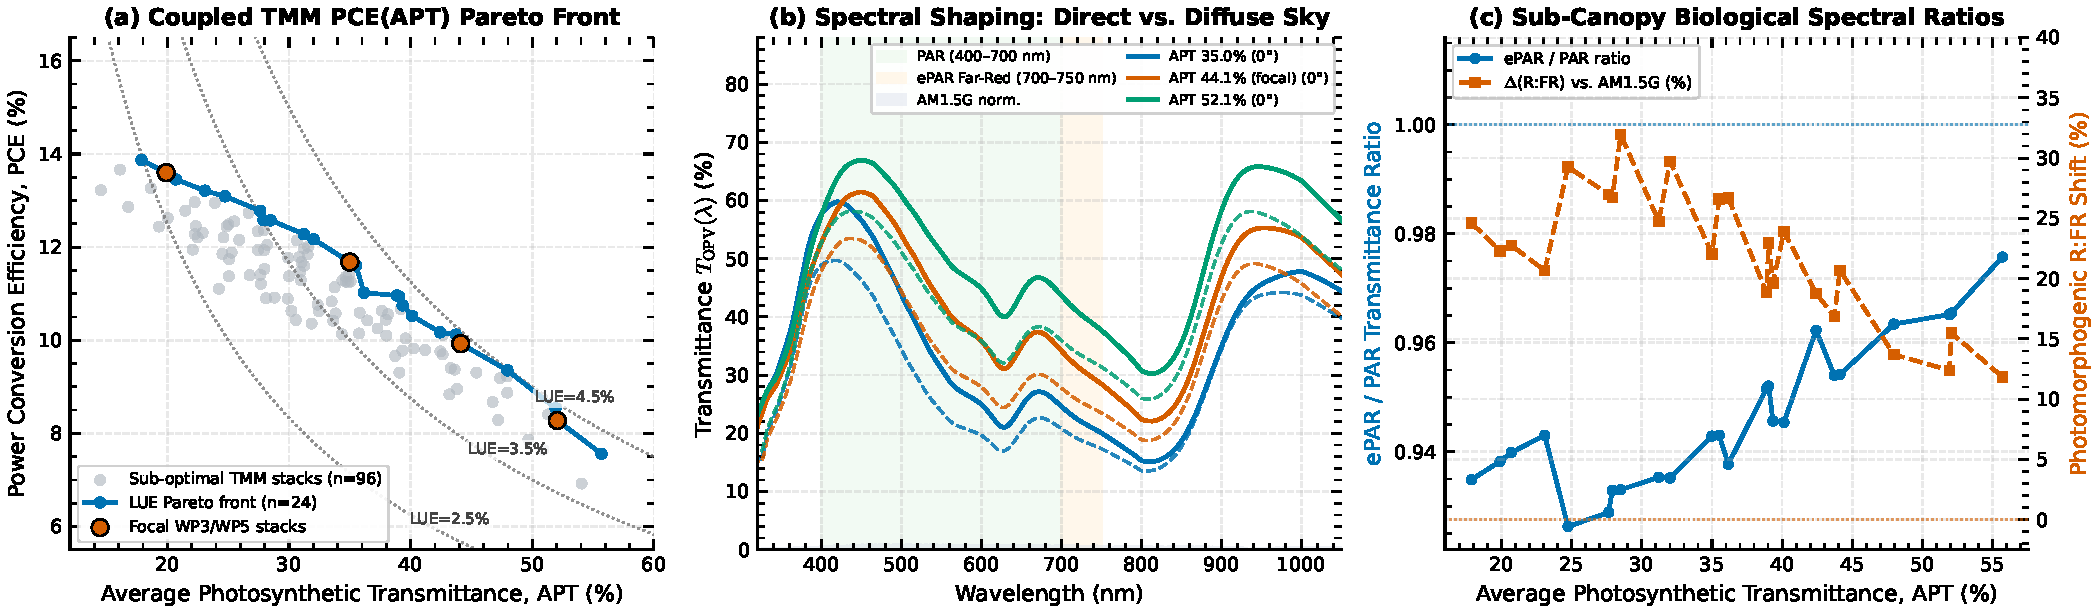
\includegraphics[width=\textwidth]{Fig1_Optical_Pareto_Spectral_TMM.pdf}
  \caption{Transfer-matrix optical design of PM6:Y6 semi-transparent organic photovoltaic (ST-OPV) canopies. (a) Coupled $\mathrm{PCE}(\mathrm{APT})$ Pareto frontier across \num{120} simulated stacks ($n=24$ Pareto optimal, $\mathrm{LUE}_{\max}=\qty{4.424}{\percent}$ in library), highlighting the four focal agrivoltaic designs ($\mathrm{APT}\approx \qty{20}{\percent}$, \qty{35}{\percent}, \qty{44.1}{\percent}, \qty{52.1}{\percent}). (b) Direct normal (\ang{0}, solid) versus diffuse hemispherical (dashed) spectral transmittance across PAR (green shading) and far-red ePAR bands (orange shading). (c) Sub-canopy $\mathrm{ePAR}/\mathrm{PAR}$ transmittance ratio and photomorphogenic $\Delta(\mathrm{R{:}FR})$ shift relative to AM1.5G.}
  \label{fig:opt_pareto}
\end{figure}

Sweeping active, metal, and capping thicknesses establishes a sharp $\mathrm{PCE}$--$\mathrm{APT}$ Pareto front bounded between $\mathrm{APT}=\qty{14.54}{\percent}$ and \qty{52.06}{\percent} ($\mathrm{LUE}_{\max}=\qty{4.424}{\percent}$ across the Pareto-optimal subset; \qty{4.486}{\percent} grid peak; \cref{fig:opt_pareto}a), while preserving photon conservation to machine precision ($\max |R + T + A_{\mathrm{tot}} - 1| = \num{4.44e-16}$) and reproducing the experimental PM6:Y6 benchmark~\cite{Shen2025NatCommun} on an opaque reference cell ($d_{\mathrm{act}}=\qty{75}{\nano\meter}$, $d_{\mathrm{Ag}}=\qty{100}{\nano\meter}$: $J_{\mathrm{sc}}=\qty{25.70}{\milli\ampere\per\square\centi\meter}$, $\mathrm{PCE}=\qty{15.50}{\percent}$ vs.\ measured \qty{26.36}{\milli\ampere\per\square\centi\meter} and \qty{16.27}{\percent}). Selecting the focal balance stack $\mathrm{APT44}$ ($d_{\mathrm{act}}=\qty{60}{\nano\meter}$, $d_{\mathrm{Ag}}=\qty{12}{\nano\meter}$, $d_{\mathrm{cap}}=\qty{35}{\nano\meter}$) achieves $\mathrm{APT}=\qty{44.12}{\percent}$ and $\mathrm{PCE}=\qty{9.93}{\percent}$ at AM1.5G, whereas thinner silver/active stacks raise transparency to $\mathrm{APT}=\qty{52.1}{\percent}$ ($\mathrm{PCE}\approx \qty{8.3}{\percent}$). Spectral transmittance curves (\cref{fig:opt_pareto}b) show pronounced blue--green transmission (\qtyrange{420}{540}{\nano\meter}, peaking above \qty{61}{\percent} for $\mathrm{APT44}$) paired with strong PM6:Y6 absorption across the red--NIR region (\qtyrange{600}{850}{\nano\meter}). Crucially, hemispherical diffuse transmittance sits \numrange{5}{10}~percentage points below \ang{0} normal beam transmittance due to higher oblique Fresnel reflection---a non-negligible penalty during humid Cameroon monsoons where diffuse sky fractions reach \qtyrange{41.6}{50.2}{\percent}. Across Pareto designs, differential attenuation near Y6's \qty{700}{\nano\meter} band edge keeps $\mathrm{ePAR}/\mathrm{PAR} \in [\num{0.926}, \num{0.976}]$ while moderately shifting transmitted $\mathrm{R{:}FR}$ by \qtyrange{+11}{+32}{\percent} (\cref{fig:opt_pareto}c).

\subsection{Microclimatic cooling, seasonal regime inversion, and four-lever attribution}
\label{sec:res_agro}

\begin{figure}[htbp]
  \centering
  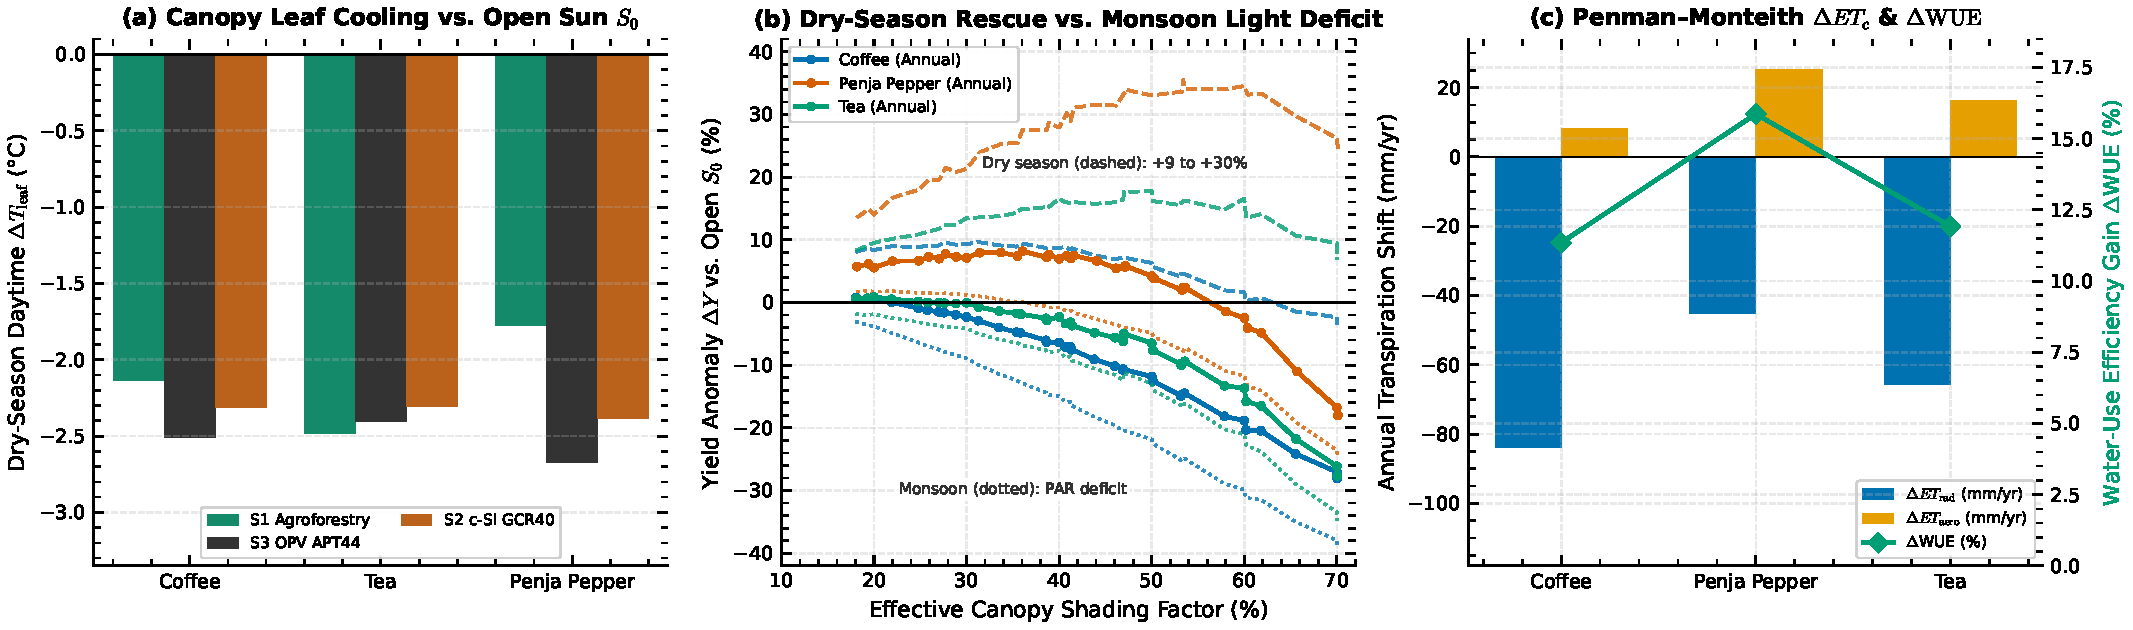
\includegraphics[width=\textwidth]{Fig3_Microclimate_Cooling_Dry_Wet_Regimes.pdf}
  \caption{Hourly ERA5 microclimate and seasonal agronomic divergence across Cameroon highlands. (a) Dry-season daytime leaf cooling ($\Delta T_{\mathrm{leaf}}$) relative to open sun $S_0$ across agroforestry ($S_1$), c-Si ($S_2$), and ST-OPV ($S_3$). (b) Annual (solid), dry-season (dashed), and monsoon wet-season (dotted) crop yield anomalies versus effective canopy shading factor. (c) Penman--Monteith radiative ($\Delta ET_{\mathrm{rad}}$) versus aerodynamic ($\Delta ET_{\mathrm{aero}}$) transpiration shifts and water-use efficiency gains ($\Delta\mathrm{WUE}$) under the focal balanced design $S_3(\mathrm{APT44,\,GCR65})$.}
  \label{fig:microclimate}
\end{figure}

\cref{fig:microclimate} and \cref{tab:agro_summary} demonstrate a decisive seasonal regime inversion across all three perennial crops. During intense dry-season midday heat, partial shading cuts canopy radiative load and cools leaves by \qtyrange{-1.51}{-2.67}{\celsius} rainfed ($\Delta T_{\mathrm{leaf}}$) and by \qtyrange{-3.10}{-3.45}{\celsius} with supplemental irrigation ($S_5$; \cref{fig:microclimate}a). Simultaneously, spectrally selective transmittance lowers daytime module self-heating on $S_3(\mathrm{APT44,\,GCR65})$ to $\Delta T_{\mathrm{PV}} = \qtyrange{3.56}{4.29}{\celsius}$ above ambient versus \qtyrange{7.73}{9.47}{\celsius} on opaque $S_2(\mathrm{c\text{-}Si,\,GCR40})$, curbing NFA efficiency derating relative to c-Si even though both systems produce similar leaf cooling (\qtyrange{-2.40}{-2.67}{\celsius} vs.\ \qtyrange{-2.31}{-2.38}{\celsius}). Because Foumbot ($\mathrm{VPD}_{95} = \qty{4.07}{\kilo\pascal}$) and Njombe-Penja ($T_{\max} = \qty{35.8}{\celsius}$) frequently cross stomatal closure and photoinhibition thresholds ($I_{\mathrm{PI}}=\qtyrange{900}{1100}{\micro\mole\per\square\meter\per\second}$), shading delivers strong dry-season yield gains under $S_3(\mathrm{APT44,\,GCR65})$ of \qty{+8.82}{\percent} (coffee), \qty{+15.98}{\percent} (tea), and \qty{+30.24}{\percent} (Penja white pepper; \cref{fig:microclimate}b, dashed curves). Simultaneously, Penman--Monteith transpiration declines (\qtyrange{-7.28}{-16.56}{\percent}) because radiative suppression ($\Delta ET_{\mathrm{rad}} = \qty{-83.98}{\milli\meter\per\yr}$ in coffee, \qty{-65.72}{\milli\meter\per\yr} in tea, and \qty{-45.29}{\milli\meter\per\yr} in pepper) dominates modest rainfed aerodynamic increases ($\Delta ET_{\mathrm{aero}} = \qtylist{+8.22;+16.41;+25.18}{\milli\meter\per\yr}$, respectively), lifting crop water-use efficiency ($\Delta\mathrm{WUE}$) by \qty{+11.35}{\percent} in coffee, \qty{+11.92}{\percent} in tea, and \qty{+15.87}{\percent} in Penja white pepper (\cref{fig:microclimate}c); adding dry-season irrigation in $S_5$ restores stomatal conductance and drives $\Delta ET_{\mathrm{aero}}$ up to \qtyrange{+43.26}{+63.17}{\milli\meter\per\yr}.

However, overcast monsoon conditions invert this mechanism: \qtyrange{36.1}{41.6}{\percent} of daytime hours under $\mathrm{GCR}=\qty{65}{\percent}$ fall into light-limited PAR regimes ($F_{\mathrm{lp}}$), inflicting wet-season yield losses of \qty{-15.88}{\percent} in Arabica coffee and \qty{-8.84}{\percent} in highland tea (\cref{fig:microclimate}b, dotted curves). Benchmarked against traditional agroforestry ($S_1$, which achieves annual shifts of \qty{-2.35}{\percent} in coffee at \qty{32.5}{\percent} shade, \qty{+7.96}{\percent} in pepper at \qty{27.5}{\percent} shade, and \qty{-1.81}{\percent} in tea at \qty{40.0}{\percent} shade), rainfed coffee under $S_3(\mathrm{APT44,\,GCR65})$ drops \qty{-7.08}{\percent} annually and tea drops \qty{-3.35}{\percent} (near neutral at \qty{-1.21}{\percent} and \qty{+0.01}{\percent} only at sparse $S_3(\mathrm{APT56,\,GCR50})$), whereas PGI Penja white pepper sustains net annual yield gains of \qty{+7.27}{\percent} under $S_3(\mathrm{APT56,\,GCR50})$, \qty{+8.16}{\percent} under $S_3(\mathrm{APT52,\,GCR65})$, and \qty{+7.43}{\percent} under $S_3(\mathrm{APT44,\,GCR65})$ (\cref{tab:agro_summary}). Heavy shading (\qty{70}{\percent} effective shade, $S_2(\mathrm{c\text{-}Si,\,GCR70})$ or $S_3(\mathrm{APT20,\,GCR85})$) imposes severe \qtyrange{-16.8}{-28.1}{\percent} yield penalties across every species. Adding dry-season supplemental irrigation in $S_5(\mathrm{APT44,\,GCR65,\,irrig.})$ rescues coffee to \qty{+0.22}{\percent} (\qty{+38.23}{\percent} dry boost), elevates tea to \qty{+2.47}{\percent} (\qty{+41.38}{\percent} dry), and propels Penja white pepper to \qty{+12.25}{\percent} (\qty{+49.68}{\percent} dry).

\begin{figure}[htbp]
  \centering
  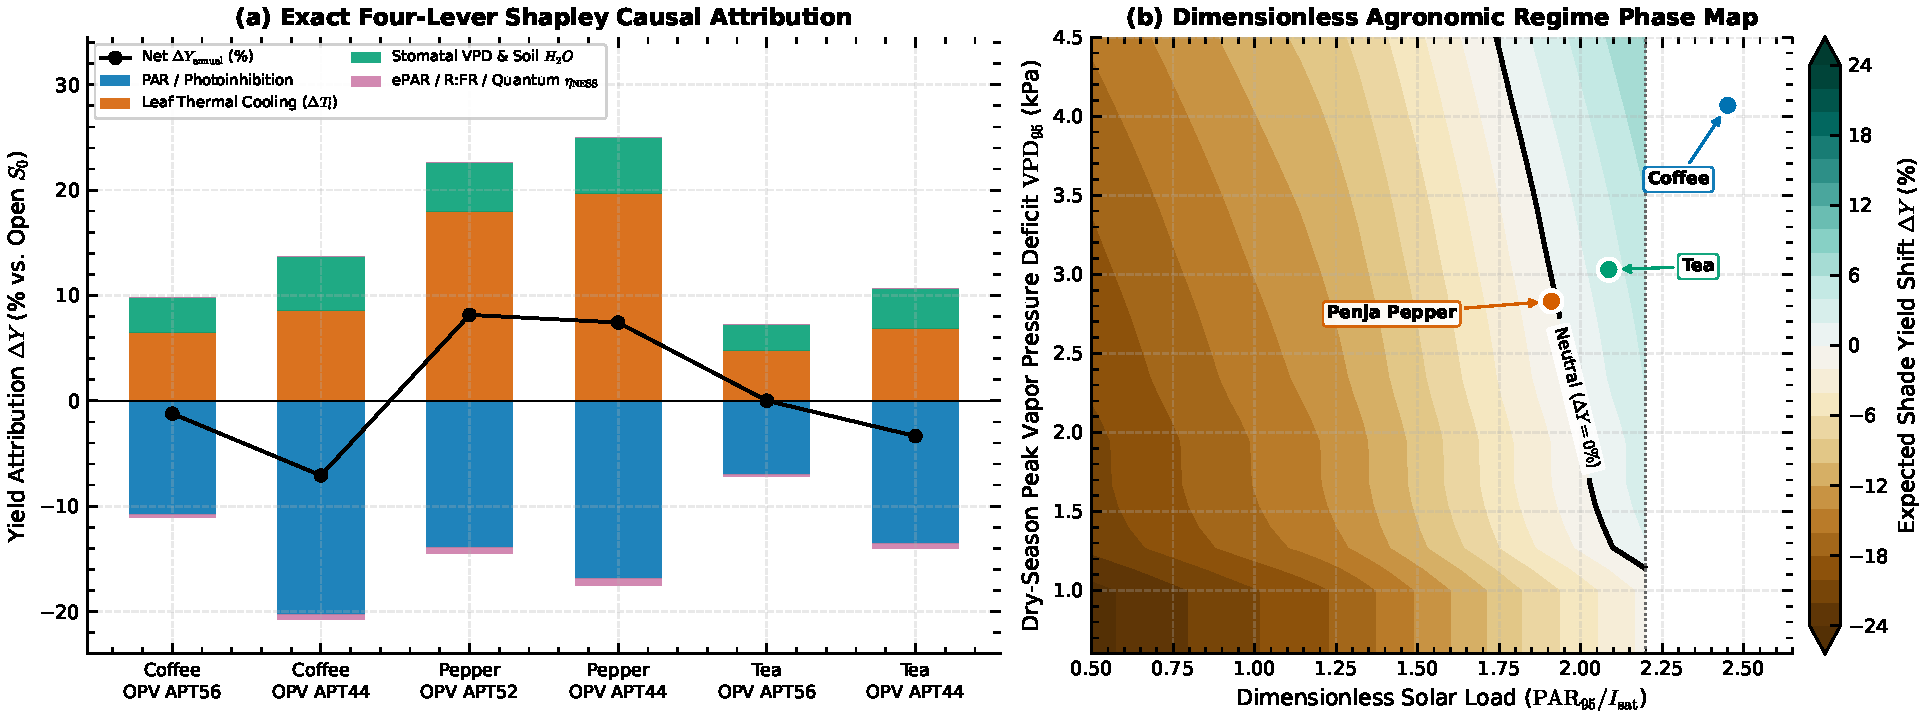
\includegraphics[width=\textwidth]{Fig4_Four_Lever_Causal_Attribution_Phase.pdf}
  \caption{Causal mechanism and climate-envelope mapping. (a) Exact 16-coalition Shapley attribution partitioning total annual yield shift $\Delta Y$ (black line) into PAR/photoinhibition, thermal leaf cooling, VPD/soil-water conservation, and spectral+quantum levers (residual $\le \qty{7.1e-15}{\percent}$). (b) Dimensionless agronomic regime phase diagram spanned by normalized dry-season solar load ($\mathrm{PAR}_{95}/I_{\mathrm{sat}}$) and $\mathrm{VPD}_{95}$, locating all three Cameroon crops near/above the neutral shade-benefit threshold.}
  \label{fig:shapley}
\end{figure}

Exact four-lever Shapley attribution (\cref{fig:shapley}a) apportions these modeled yield responses across physical mechanisms. For Penja white pepper under $S_3(\mathrm{APT52,\,GCR65})$ (\qty{+8.16}{\percent}), thermal leaf cooling (\qty{+17.99}{\percent}) and stomatal/soil moisture conservation (\qty{+4.64}{\percent}) outweigh the PAR reduction penalty (\qty{-13.93}{\percent}), while optical spectral quality plus quantum NESS ($\phi_{\mathrm{spec+Q}} = \qty{-0.55}{\percent}$) play a minor sub-percent role. Conversely, in Foumbot coffee under $S_3(\mathrm{APT44,\,GCR65})$ (\qty{-7.08}{\percent}), the PAR penalty (\qty{-20.31}{\percent}) dominates combined thermal (\qty{+8.58}{\percent}) and soil-water (\qty{+5.11}{\percent}) gains. Directly comparing ST-OPV and elevated c-Si at matched $\sim\qty{40}{\percent}$ shade ($S_3(\mathrm{APT44,\,GCR65})$ vs.\ $S_2(\mathrm{c\text{-}Si,\,GCR40})$; \cref{tab:agro_summary}) reveals nearly indistinguishable annual crop yields---differing by at most \num{1.05}~percentage points (\qty{-7.08}{\percent} vs.\ \qty{-6.38}{\percent} in coffee, \qty{+7.43}{\percent} vs.\ \qty{+6.95}{\percent} in pepper, \qty{-3.35}{\percent} vs.\ \qty{-2.30}{\percent} in tea). Across all ST-OPV designs ($\mathrm{APT56}$--$\mathrm{APT44}$), $\phi_{\mathrm{spec+Q}}$ contributes only \qtyrange{-0.21}{-0.67}{\percent} (slightly negative because PM6:Y6 band-edge absorption reduces the transmitted $\mathrm{ePAR}/\mathrm{PAR}$ ratio below open sunlight), indicating within the coupled model that total shade fraction and wet--dry seasonality, rather than spectral selectivity, govern agronomic performance. The matched-shade design equalizes only the crop-light service, not the useful-energy service: across the ten weather years the focal ST-OPV canopy delivers \qtyrange{975}{1193}{\MWh\per\hectare\per\yr} against \qtyrange{1179}{1447}{\MWh\per\hectare\per\yr} for $S_2(\mathrm{c\text{-}Si,\,GCR40})$ (pepper-to-coffee range), i.e. \qtyrange{81.2}{82.8}{\percent} of the opaque counterfactual's generation at matched $\sim\qty{40}{\percent}$ shade (a deficit of \qtyrange{203}{254}{\MWh\per\hectare\per\yr}; \qtyrange{81.0}{83.0}{\percent} in the 2023 baseline). This gap combines the $\sim\qty{40}{\percent}$ of incident PAR deliberately transmitted to the crop layer with the reference module efficiencies (\qty{9.93}{\percent} PM6:Y6 vs.\ \qty{20.5}{\percent} c-Si). No configuration in the design set pairs equal energy with equal shade: an energy-matched c-Si array would sit near $\mathrm{GCR}\,30$--$35$ with correspondingly lower shade, trading crop-light parity for energy parity. The comparative $\Delta\mathrm{NPV}$ therefore contrasts equal crop-light service with unequal useful-energy service---partly pricing this $\sim\qty{18}{\percent}$ generation gap into c-Si's dominance in \qtyrange{77}{89}{\percent} of draws---and the two services should not be read as jointly matched. Mapping peak irradiance normalized by species saturation ($I_{\mathrm{sat}}$) against $\mathrm{VPD}_{95}$ (\cref{fig:shapley}b) highlights the narrow envelope governing annual rainfed viability without dynamic tracking.

\begin{table}[htbp]
  \centering
  \caption{Focal seasonal agronomic performance, exact four-lever Shapley decomposition ($\phi_i$), water-use shift ($\Delta\mathrm{WUE}$), and annual PV yield across Cameroon perennials.}
  \label{tab:agro_summary}
  \scriptsize
  \resizebox{\textwidth}{!}{
\begin{tabular}{@{}llrrrrrrrrr@{}}
    \toprule
    \textbf{Crop} & \textbf{Scenario} & \textbf{Shade} & $\Delta Y_{\mathrm{ann}}$ & $\Delta Y_{\mathrm{dry}}$ & $\Delta Y_{\mathrm{wet}}$ & $\phi_{\mathrm{PAR/PI}}$ & $\phi_{\mathrm{therm}}$ & $\phi_{\mathrm{H_2O}}$ & $\Delta\mathrm{WUE}$ & \textbf{PV} \\
    & & (\unit{\percent}) & (\unit{\percent}) & (\unit{\percent}) & (\unit{\percent}) & (\unit{\percent}) & (\unit{\percent}) & (\unit{\percent}) & (\unit{\percent}) & (\unit{\MWh\per\hectare}) \\
    \midrule
    Coffee & S3 (APT56, GCR50) & \num{25.7} & \num{-1.21} & \num{+9.02} & \num{-6.96} & \num{-10.82} & \num{+6.45} & \num{+3.37} & \num{+7.80} & \num{717.0} \\
    Coffee & S3 (APT44, GCR65) & \num{40.6} & \num{-7.08} & \num{+8.82} & \num{-15.88} & \num{-20.31} & \num{+8.58} & \num{+5.11} & \num{+11.35} & \num{1223.3} \\
    Coffee & S5 (APT44, GCR65, irrig.) & \num{40.6} & \num{+0.22} & \num{+38.23} & \num{-15.88} & \num{-21.38} & \num{+10.81} & \num{+11.25} & \num{+0.15} & \num{1223.3} \\
    Coffee & S2 (c-Si, GCR40) & \num{40.0} & \num{-6.38} & \num{+8.73} & \num{-14.92} & \num{-19.24} & \num{+8.14} & \num{+4.71} & \num{+9.56} & \num{1479.0} \\
    \midrule
    Pepper & S3 (APT56, GCR50) & \num{25.9} & \num{+7.27} & \num{+19.57} & \num{+1.53} & \num{-8.73} & \num{+13.25} & \num{+3.02} & \num{+11.19} & \num{611.7} \\
    Pepper & S3 (APT52, GCR65) & \num{36.0} & \num{+8.16} & \num{+27.56} & \num{+0.04} & \num{-13.93} & \num{+17.99} & \num{+4.64} & \num{+15.19} & \num{870.2} \\
    Pepper & S3 (APT44, GCR65) & \num{40.8} & \num{+7.43} & \num{+30.24} & \num{-1.36} & \num{-16.87} & \num{+19.69} & \num{+5.27} & \num{+15.87} & \num{1043.7} \\
    Pepper & S5 (APT44, GCR65, irrig.) & \num{40.8} & \num{+12.25} & \num{+49.68} & \num{-1.36} & \num{-17.06} & \num{+21.56} & \num{+8.40} & \num{+9.02} & \num{1043.7} \\
    Pepper & S2 (c-Si, GCR40) & \num{40.0} & \num{+6.95} & \num{+27.89} & \num{-0.78} & \num{-15.72} & \num{+17.90} & \num{+4.75} & \num{+12.11} & \num{1257.2} \\
    \midrule
    Tea & S3 (APT56, GCR50) & \num{25.8} & \num{+0.01} & \num{+11.26} & \num{-3.47} & \num{-6.99} & \num{+4.73} & \num{+2.48} & \num{+8.29} & \num{652.5} \\
    Tea & S3 (APT44, GCR65) & \num{40.7} & \num{-3.35} & \num{+15.98} & \num{-8.84} & \num{-13.53} & \num{+6.84} & \num{+3.86} & \num{+11.92} & \num{1113.3} \\
    Tea & S5 (APT44, GCR65, irrig.) & \num{40.7} & \num{+2.47} & \num{+41.38} & \num{-8.84} & \num{-13.90} & \num{+8.36} & \num{+8.50} & \num{+0.74} & \num{1113.3} \\
    Tea & S2 (c-Si, GCR40) & \num{40.0} & \num{-2.30} & \num{+16.56} & \num{-7.65} & \num{-12.63} & \num{+6.65} & \num{+3.68} & \num{+10.77} & \num{1374.4} \\
    \bottomrule
  \end{tabular}
}
\end{table}

\subsection{Cooperative dispatch, dual-FU LCA, and break-even frontiers}
\label{sec:res_tea}

\begin{figure}[htbp]
  \centering
  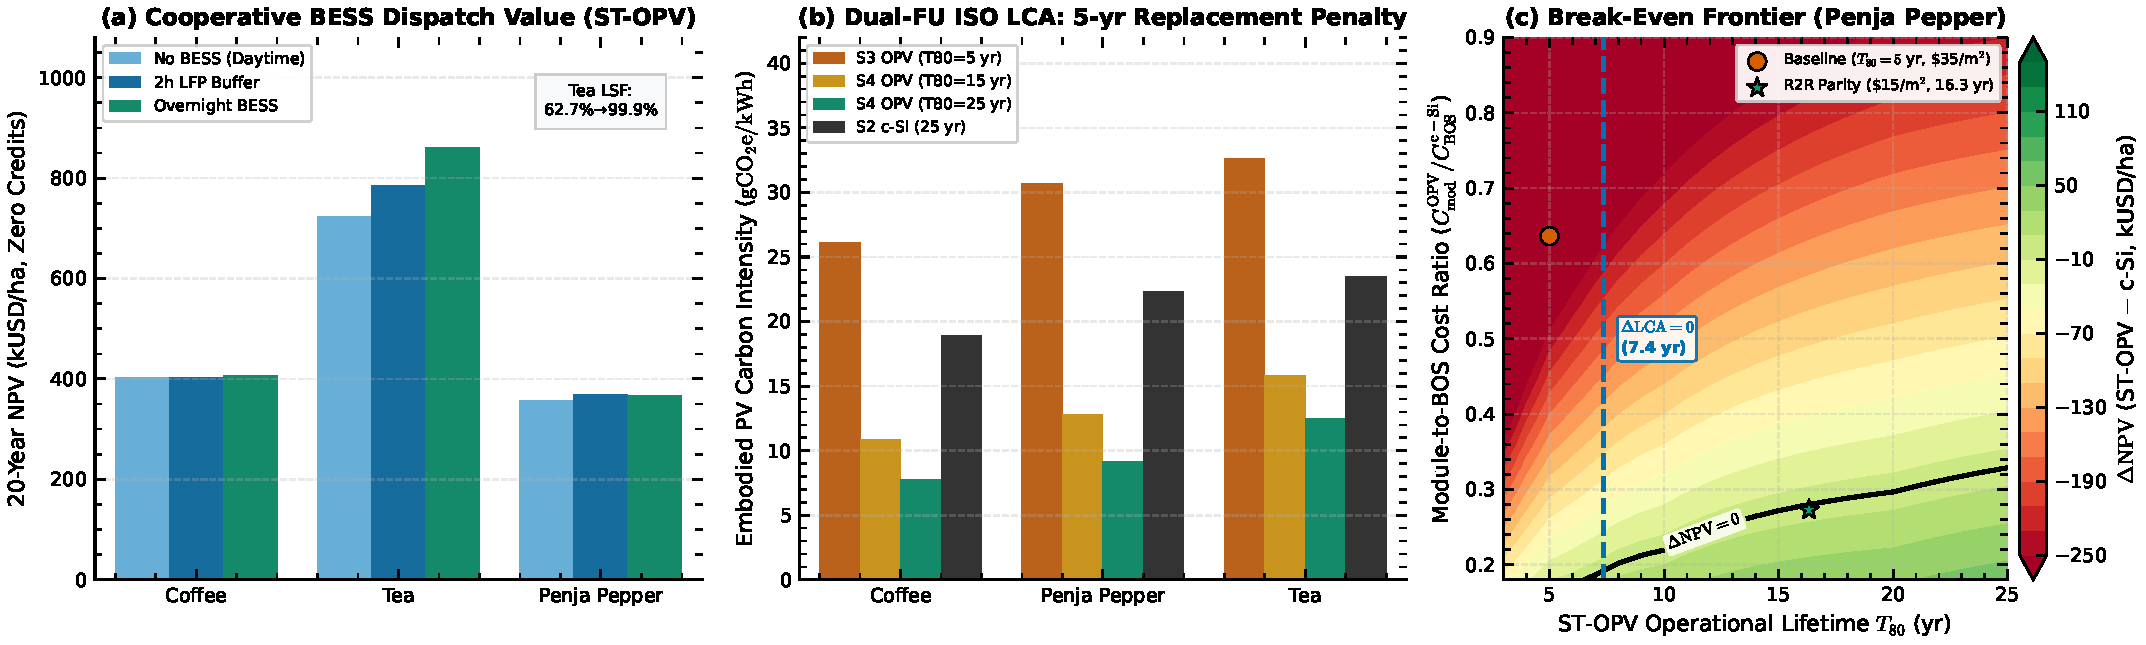
\includegraphics[width=\textwidth]{Fig5_Dispatch_TEA_LCA_BreakEven.pdf}
  \caption{Techno-economic dispatch, environmental carbon intensity, and parity thresholds (\qty{0}{\USD\per\tCOtwoe}, \qty{0}{\percent} subsidy baseline). (a) Effect of LFP storage sizing on \qty{20}{\yr} NPV for $S_3(\mathrm{APT44,\,GCR65})$, highlighting Djuttitsa tea load solar fraction ($\mathrm{LSF}$) climbing from \qty{62.7}{\percent} to \qty{99.9}{\percent}. (b) Embodied PV carbon intensity across \qty{5}{\yr} ($S_3$), \qty{15}{\yr} / \qty{25}{\yr} encapsulated ST-OPV ($S_4$), and \qty{25}{\yr} c-Si ($S_2$). (c) Two-dimensional NPV and LCA parity frontier over ST-OPV operational lifetime ($T_{80}$) and module-to-BOS cost ratio for Penja white pepper.}
  \label{fig:tea_lca}
\end{figure}

Integrating cooperative processing dispatch fundamentally differentiates Djuttitsa tea from daytime-dominated coffee and pepper cooperatives (\cref{fig:tea_lca}a, \cref{tab:tea_lca}). Because tea withering consumes \qty{45}{\percent} of its \qty{307.8}{\MWh\per\yr} factory electricity overnight, shifting from daytime-only operation without storage to overnight-withering LFP storage boosts load solar fraction from \qty{62.68}{\percent} to \qty{99.92}{\percent} and raises \qty{20}{\yr} NPV from \qty{724075}{\USD\per\hectare} ($\mathrm{IRR} = \qty{38.65}{\percent}$) to \qty{860825}{\USD\per\hectare} ($\mathrm{IRR} = \qty{35.52}{\percent}$, $\mathrm{DPBP} = \qty{3.01}{\yr}$, $\mathrm{LCOE} = \qty{0.0886}{\USD\per\kWh}$), delivering \qty{393.2}{\tCOtwoe\per\hectare\per\yr} in net areal carbon abatement after accounting for amortized embodied and on-farm diesel emissions (equivalent to \qty{427.3}{\tCOtwoe\per\hectare\per\yr} in gross displaced grid and diesel electricity). By contrast, Foumbot coffee and Njombe-Penja pepper cooperatives run primarily during daytime hours ($\mathrm{LSF} = \qtyrange{88.6}{92.4}{\percent}$ without storage), gaining negligible incremental value from overnight BESS ($\mathrm{NPV} = \qtyrange{402.5}{406.9}{\kUSD\per\hectare}$ coffee, $\mathrm{DPBP} = \qty{3.95}{\yr}$ with \qty{2}{\hour} buffer; \qtyrange{358.0}{368.4}{\kUSD\per\hectare} pepper, $\mathrm{DPBP} = \qty{5.73}{\yr}$ vs.\ \qty{3.52}{\yr} and \qty{3.80}{\yr} on elevated c-Si).

Under a dual-functional-unit ISO~14040/14044 assessment ($T_{80}=\qty{5}{\yr}$ baseline; \cref{fig:tea_lca}b), frequent ST-OPV replacement drives embodied intensity (\qtyrange{26.1}{32.7}{\gCOtwoe\per\kWh}) above single-install \qty{25}{\yr} c-Si (\qtyrange{18.9}{23.5}{\gCOtwoe\per\kWh}). Extending encapsulated NFA lifetime breaks environmental parity cleanly at $T_{80,\mathrm{LCA}}^* = \qty{7.42}{\yr}$ (coffee), \qty{7.40}{\yr} (Penja pepper), and \qty{8.12}{\yr} (tea). Under $S_4$ encapsulation ($T_{80}=\qtyrange{15}{25}{\yr}$ at baseline CAPEX), ST-OPV carbon intensity falls by \qtyrange{51}{70}{\percent} to \qtyrange{10.8}{15.9}{\gCOtwoe\per\kWh} at \qty{15}{\yr} and \qtyrange{7.8}{12.5}{\gCOtwoe\per\kWh} at \qty{25}{\yr} (less than half c-Si intensity), LCOE declines by \qtyrange{23.1}{33.8}{\percent} down to \qtylist{0.0422;0.0497;0.0646}{\USD\per\kWh}, $\mathrm{DPBP}$ tightens to \qtylist{3.76;3.94;2.91}{\yr}, and annualized net areal abatement rises to \qty{334.5}{\tCOtwoe\per\hectare\per\yr} (coffee), \qty{296.7}{\tCOtwoe\per\hectare\per\yr} (pepper), and \qty{412.5}{\tCOtwoe\per\hectare\per\yr} (tea). However, economic parity is far more stringent (\cref{fig:tea_lca}c): at current \qty{35}{\USD\per\square\meter} module pricing, ST-OPV never reaches financial parity with c-Si within \qty{30}{\yr} ($T_{80,\mathrm{NPV}}^* > \qty{30}{\yr}$ across all three crops) because elevated c-Si generates \qtyrange{21}{24}{\percent} more electricity per hectare (\qtyrange{1257}{1479}{\MWh\per\hectare\per\yr} vs.\ \qtyrange{1044}{1223}{\MWh\per\hectare\per\yr}). Only once roll-to-roll manufacturing compresses module CAPEX to \qty{15}{\USD\per\square\meter} ($C_{\mathrm{mod}}^{\mathrm{OPV}} / C_{\mathrm{BOS}}^{\mathrm{c\text{-}Si}} = \num{0.273}$) does NPV parity emerge at $T_{80,\mathrm{NPV}}^* = \qty{16.33}{\yr}$ for Penja white pepper and \qty{31.27}{\yr} for coffee, whereas tea remains c-Si favored ($T_{80,\mathrm{NPV}}^* > \qty{30}{\yr}$) due to high captive electricity value per installed $\mathrm{W_p}$.

\begin{table}[htbp]
  \centering
  \caption{Techno-economic and life-cycle comparison ($S_3(\mathrm{APT44,\,GCR65})$ vs.\ $S_2(\mathrm{c\text{-}Si,\,GCR40})$) and break-even thresholds at the strict zero-subsidy baseline (\qty{0}{\USD\per\tCOtwoe}, $\mathrm{WACC} = \qty{10}{\percent}$).}
  \label{tab:tea_lca}
  \scriptsize
  \resizebox{\textwidth}{!}{
\begin{tabular}{@{}llrrrrrrr@{}}
    \toprule
    \textbf{Crop} & \textbf{System / Dispatch} & \textbf{LSF} & \textbf{LER} & \textbf{NPV} & \textbf{IRR} & \textbf{LCOE} & \textbf{LCA} & \textbf{Off-Grid NPV} \\
    & & (\unit{\percent}) & (--) & (\unit{\kUSD\per\hectare}) & (\unit{\percent}) & (\unit{\USD\per\kWh}) & (\unit{\gCOtwoe\per\kWh}) & (\unit{\kUSD\per\hectare}) \\
    \midrule
    Coffee & ST-OPV (no BESS) & \num{92.42} & \num{1.401} & \num{402.5} & \num{26.46} & \num{0.0625} & \num{25.90} & -- \\
    Coffee & ST-OPV (\qty{2}{\hour} BESS) & \num{100.00} & \num{1.401} & \num{403.5} & \num{26.16} & \num{0.0637} & \num{26.16} & \num{-379.8} \\
    Coffee & c-Si (\qty{2}{\hour} BESS) & \num{100.00} & \num{1.507} & \num{779.3} & \num{34.77} & \num{0.0380} & \num{18.92} & -- \\
    \midrule
    Penja Pepper & ST-OPV (no BESS) & \num{88.62} & \num{1.548} & \num{358.0} & \num{24.72} & \num{0.0733} & \num{30.36} & -- \\
    Penja Pepper & ST-OPV (\qty{2}{\hour} BESS) & \num{99.97} & \num{1.548} & \num{368.4} & \num{24.74} & \num{0.0750} & \num{30.73} & \num{-281.5} \\
    Penja Pepper & c-Si (\qty{2}{\hour} BESS) & \num{99.99} & \num{1.640} & \num{709.1} & \num{32.55} & \num{0.0449} & \num{22.31} & -- \\
    \midrule
    Highland Tea & ST-OPV (no BESS) & \num{62.68} & \num{1.429} & \num{724.1} & \num{38.65} & \num{0.0687} & \num{28.46} & -- \\
    Highland Tea & ST-OPV (\qty{2}{\hour} BESS) & \num{74.30} & \num{1.429} & \num{785.7} & \num{39.02} & \num{0.0727} & \num{29.32} & -- \\
    Highland Tea & ST-OPV (overnight BESS) & \num{99.92} & \num{1.429} & \num{860.8} & \num{35.52} & \num{0.0886} & \num{32.66} & \num{+319.8} \\
    Highland Tea & c-Si (overnight BESS) & \num{100.00} & \num{1.548} & \num{1272.6} & \num{41.66} & \num{0.0555} & \num{23.46} & -- \\
    \bottomrule
  \end{tabular}
}
\end{table}

\subsection{Sobol uncertainty quantification and policy stress tests}
\label{sec:res_sobol}

\begin{figure}[htbp]
  \centering
  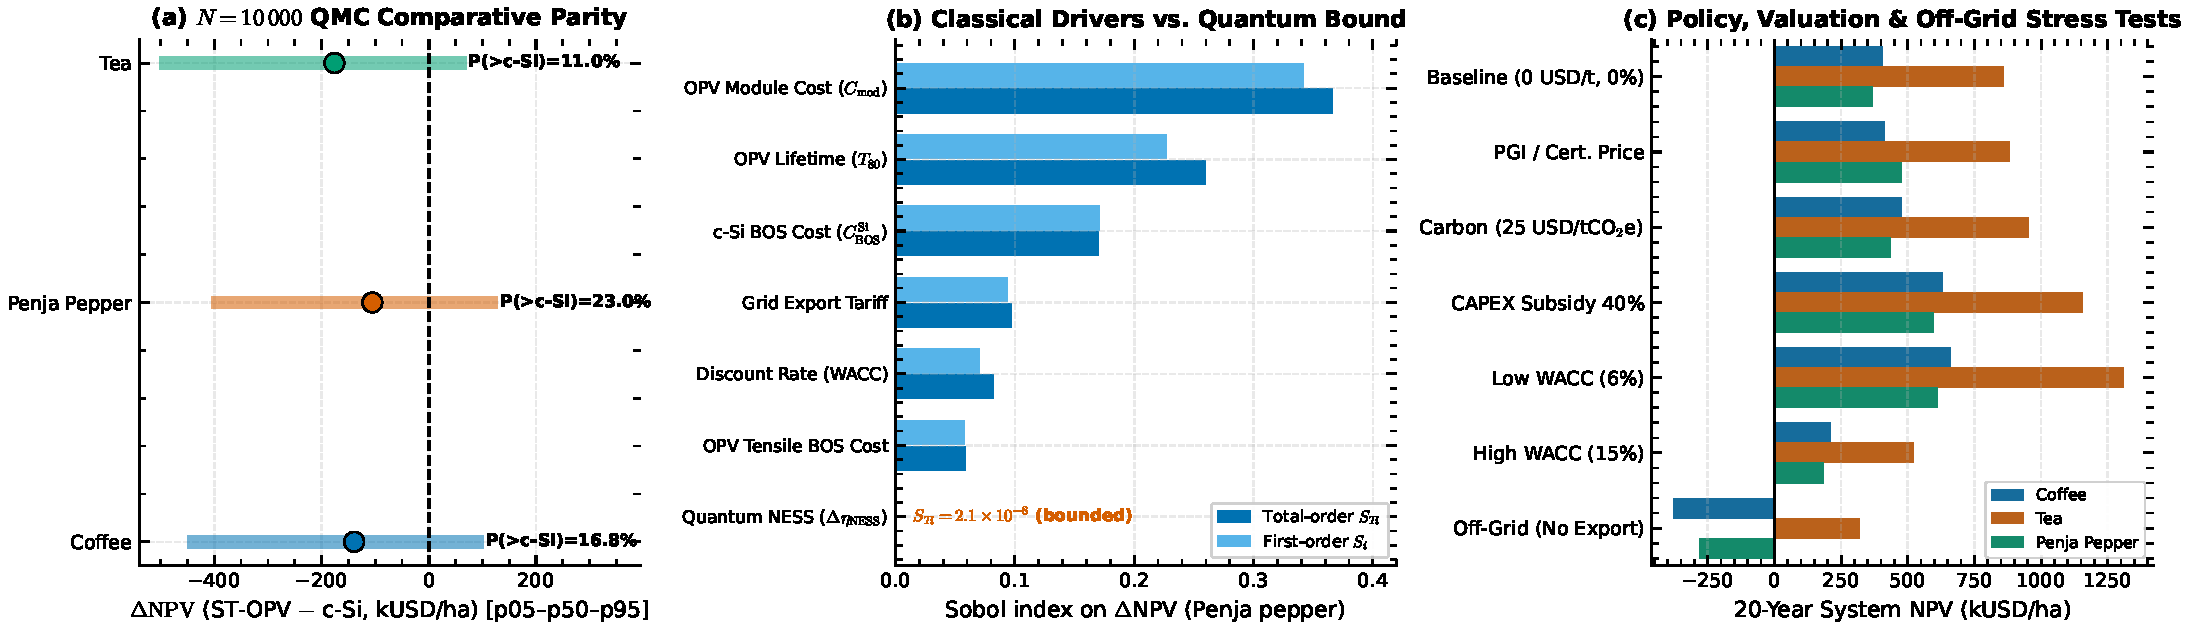
\includegraphics[width=\textwidth]{Fig6_Sobol_Uncertainty_LER_Policy.pdf}
  \caption{Probabilistic parity and global variance attribution ($N = \num{10000}$ Saltelli QMC draws). (a) Comparative $\Delta\mathrm{NPV} = \mathrm{NPV}_{\mathrm{OPV}} - \mathrm{NPV}_{\mathrm{Si}}$ [p05--p50--p95] distributions and exceedance probabilities. (b) Ranked first-order ($S_i$) and total-order ($S_{Ti}$) Sobol indices on Penja white pepper $\Delta\mathrm{NPV}$ alongside the bounded quantum NESS index ($S_{Ti} = \num{2.10e-8}$; $\le \num{2.58e-7}$ under the exact-HEOM envelope). (c) Policy, valuation, discount-rate, and off-grid stress tests across the three crops ($S_3(\mathrm{APT44,\,GCR65})$).}
  \label{fig:sobol}
\end{figure}

Across $N=\num{10000}$ Saltelli quasi-Monte Carlo parameter realizations spanning the full 12-parameter policy and techno-economic uncertainty box (carbon pricing $[\num{0}, \num{25}]\,\unit{\USD\per\tCOtwoe}$; \cref{fig:sobol}a), ST-OPV exceeds elevated c-Si NPV in only \qty{22.99}{\percent} of Penja white pepper draws (median \qty{-105.3}{\kUSD\per\hectare}, p05--p95 \qtyrange{-394.4}{+116.9}{\kUSD\per\hectare}), \qty{16.75}{\percent} of Arabica coffee draws (median \qty{-139.3}{\kUSD\per\hectare}, \qtyrange{-437.6}{+90.2}{\kUSD\per\hectare}), and \qty{11.00}{\percent} of tea draws (median \qty{-176.0}{\kUSD\per\hectare}, \qtyrange{-490.0}{+58.0}{\kUSD\per\hectare}), meaning elevated c-Si dominates in \qtyrange{77.0}{89.0}{\percent} of realizations. Under strict zero-carbon pricing (\qty{0}{\USD\per\tCOtwoe}), ST-OPV exceedance rises only slightly to \qty{24.71}{\percent} for pepper (median \qty{-97.9}{\kUSD\per\hectare}), \qty{18.51}{\percent} for coffee (median \qty{-131.0}{\kUSD\per\hectare}), and \qty{12.34}{\percent} for tea (median \qty{-166.5}{\kUSD\per\hectare}), confirming that carbon credits slightly favor higher-output c-Si rather than rescuing ST-OPV ($S_{Ti} \le \num{0.0011}$).

Contrast of Saltelli--Sobol total-order indices between standalone ST-OPV profitability ($\mathrm{NPV}_{\mathrm{OPV}}$) and comparative parity ($\Delta\mathrm{NPV}$) exposes a clear Dual Policy Bifurcation (\cref{tab:sobol_dual}, \cref{fig:sobol}b). Even though standalone ST-OPV installations remain consistently profitable across policy realizations (p05--p50--p95 spanning \qtylist{145.0;562.3;1116.5}{\kUSD\per\hectare} in coffee; \qtylist{148.4;537.8;1038.5}{\kUSD\per\hectare} in pepper; and \qtylist{505.6;1042.8;1780.2}{\kUSD\per\hectare} in tea), project bankability in daytime-dominated coffee and pepper is governed by grid export tariff ($S_{Ti}=\num{0.5176}$ and \num{0.4263}) and cost of capital WACC ($S_{Ti}=\num{0.2866}$ and \num{0.3198}), whereas energy-intensive tea processing reverses this hierarchy to WACC ($S_{Ti}=\num{0.4503}$) and displaced diesel price ($S_{Ti}=\num{0.2817}$) ahead of export tariff (\num{0.1471}). Once technology selection $\Delta\mathrm{NPV}$ is evaluated at equal shade, shared macroeconomic parameters largely cancel, transferring over \qty{74}{\percent} of cumulative variance to three hardware levers: OPV module CAPEX ($S_{Ti}=\numrange{0.323}{0.366}$, peaking at \num{0.3663} in pepper), ST-OPV $T_{80}$ lifetime ($S_{Ti}=\numrange{0.247}{0.267}$), and c-Si elevated steel BOS CAPEX ($S_{Ti}=\numrange{0.150}{0.170}$).

\begin{table}[htbp]
  \centering
  \caption{Dual Saltelli--Sobol decomposition ($N=\num{10000}$ base samples, \num{140000} evaluations per crop) contrasting macro-financial drivers of standalone bankability ($\mathrm{NPV}_{\mathrm{OPV}}$) against hardware engineering drivers of comparative parity ($\Delta\mathrm{NPV} = \mathrm{NPV}_{\mathrm{OPV}} - \mathrm{NPV}_{\mathrm{Si}}$).}
  \label{tab:sobol_dual}
  \scriptsize
  \resizebox{\textwidth}{!}{
  \begin{tabular}{@{}lclrrlc@{}}
    \toprule
    \textbf{Crop} & $\mathrm{NPV}_{\mathrm{OPV}}^{p50}$ $[p05, p95]$ & \textbf{Top $S_{Ti}(\mathrm{NPV}_{\mathrm{OPV}})$ drivers} & $P(\Delta>0)$ & $\Delta\mathrm{NPV}_{p50}$ & \textbf{Top $S_{Ti}(\Delta\mathrm{NPV})$ drivers} & $S_{Ti}^Q$ ($\mathrm{NPV}_{\mathrm{OPV}}$ / $\Delta\mathrm{NPV}$) \\
     & (\unit{\kUSD\per\hectare}) & (parameter, index) & (\unit{\percent}) & (\unit{\kUSD\per\hectare}) & (parameter, index) & (--) \\
    \midrule
    Arabica coffee & \num{562.3} [\num{145.0}, \num{1116.5}] & Tariff (\num{0.518}), WACC (\num{0.287}), $C_{\mathrm{mod}}^{\mathrm{OPV}}$ (\num{0.104}) & \num{16.75} & \num{-139.3} & $C_{\mathrm{mod}}^{\mathrm{OPV}}$ (\num{0.343}), $T_{80}$ (\num{0.247}), $C_{\mathrm{BOS}}^{\mathrm{c\text{-}Si}}$ (\num{0.159}) & \num{1.16e-9} / \num{3.83e-9} \\
    Penja white pepper & \num{537.8} [\num{148.4}, \num{1038.5}] & Tariff (\num{0.426}), WACC (\num{0.320}), $C_{\mathrm{mod}}^{\mathrm{OPV}}$ (\num{0.125}) & \num{22.99} & \num{-105.3} & $C_{\mathrm{mod}}^{\mathrm{OPV}}$ (\num{0.366}), $T_{80}$ (\num{0.260}), $C_{\mathrm{BOS}}^{\mathrm{c\text{-}Si}}$ (\num{0.170}) & \num{7.15e-9} / \num{2.10e-8} \\
    Highland tea & \num{1042.8} [\num{505.6}, \num{1780.2}] & WACC (\num{0.450}), Diesel (\num{0.282}), Tariff (\num{0.147}) & \num{11.00} & \num{-176.0} & $C_{\mathrm{mod}}^{\mathrm{OPV}}$ (\num{0.323}), $T_{80}$ (\num{0.267}), $C_{\mathrm{BOS}}^{\mathrm{c\text{-}Si}}$ (\num{0.150}) & \num{1.89e-9} / \num{9.85e-9} \\
    \bottomrule
  \end{tabular}
  }
\end{table}

Policy stress tests (\cref{fig:sobol}c) reinforce this dispatch-dependent bifurcation under grid isolation: removing grid export drops NPV to \qty{-379.8}{\kUSD\per\hectare} in coffee and \qty{-281.5}{\kUSD\per\hectare} in Penja pepper because captive spice and pulping demand absorbs $< \qty{10}{\percent}$ of array output, whereas Djuttitsa tea stays strongly profitable at \qty{+319794}{\USD\per\hectare} ($\mathrm{IRR} = \qty{20.06}{\percent}$, $\mathrm{DPBP}=\qty{6.61}{\yr}$). Certified PGI pricing (\qty{14000}{\XAF\per\kilogram}) adds $\sim\qty{100}{\kUSD\per\hectare}$ to Penja white pepper NPV, while concessional capital ($\mathrm{WACC} = \qty{6}{\percent}$) matches a \qty{40}{\percent} upfront CAPEX grant in raising system NPV across all basins.

% ==============================================================================
\section{Quantum-to-system boundary analysis: pulsed coherent dynamics vs.\ CW sunlight}
\label{sec:quantum_bound}
% ==============================================================================

\begin{figure}[htbp]
  \centering
  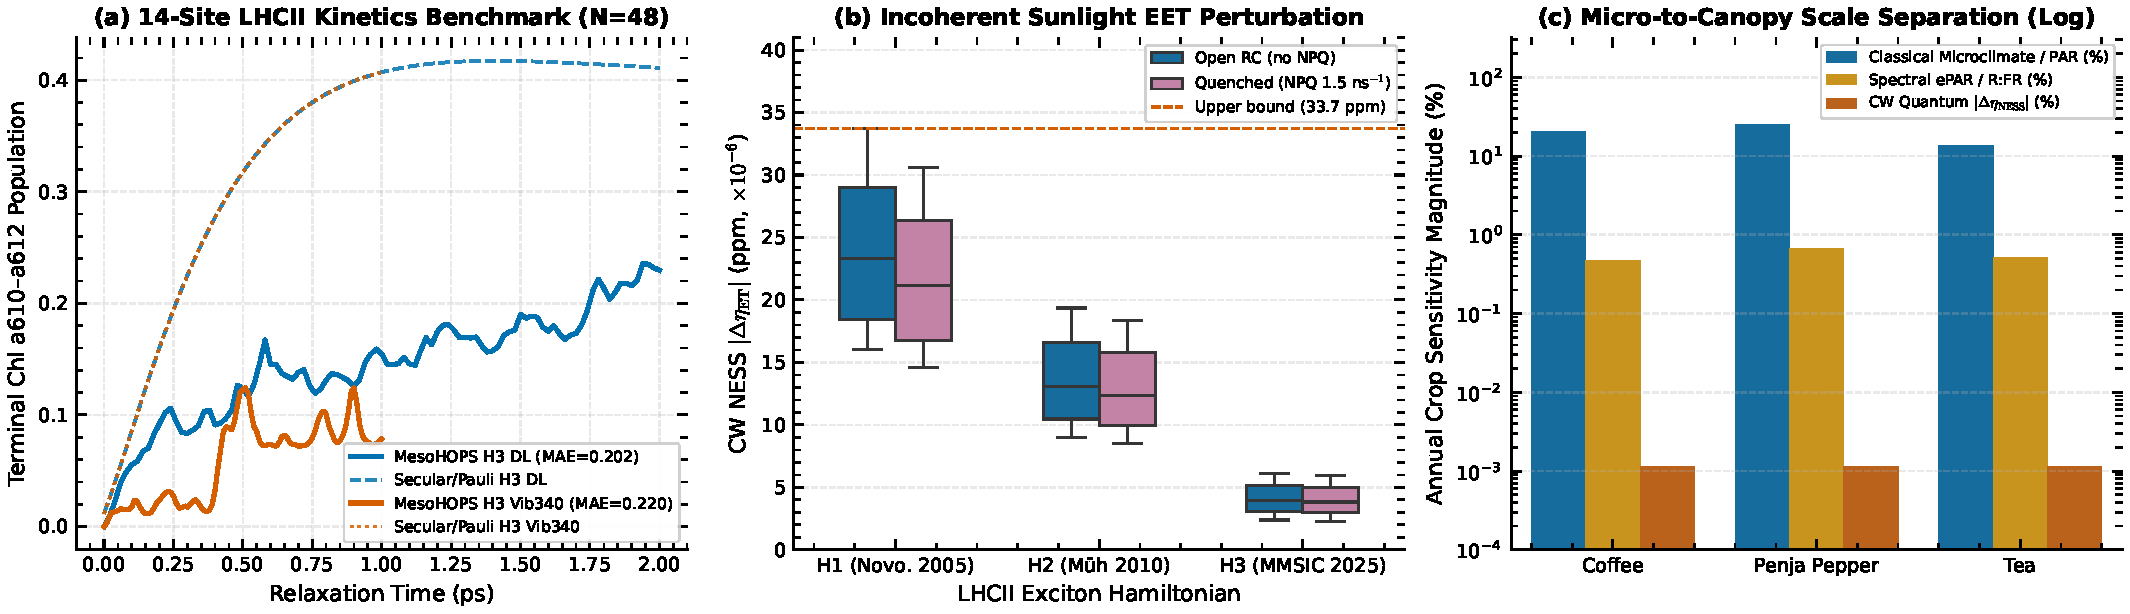
\includegraphics[width=\textwidth]{Fig2_Quantum_NESS_Bound_Benchmark.pdf}
  \caption{Microscopic open-quantum light-harvesting validation and canopy scale separation. (a) Full non-Markovian 14-site MesoHOPS~1.8.0 pulsed excitation kinetics ($N = 48$ disorder draws, $T=\qty{295}{\kelvin}$) versus diagonal secular Pauli kinetics on H3 (Drude--Lorentz bath alone to \qty{2.0}{\pico\second} and augmented with the \qty{340}{\per\centi\meter} vibronic mode to \qty{1.0}{\pico\second}). (b) Continuous-wave (CW) solar NESS perturbation $|\Delta\eta_{\mathrm{ET}}|$ across all ST-OPV transmittance spectra (\ang{0} beam and diffuse) and three independent LHCII Hamiltonians (H1--H3), strictly bounded at \qty{33.7}{\ppm} (\num{3.37e-5}). (c) Log-scale comparison of annual canopy crop sensitivity magnitudes ($\sim\qty{10}{\percent}$ microclimate vs.\ $\sim\qty{e-3}{\percent}$ maximum quantum EET shift).}
  \label{fig:quantum}
\end{figure}

Answering the second half of our central research question requires establishing precisely where coherent quantum biology matters and where it rigorously decouples. On ultrafast pulsed timescales representative of 2D electronic spectroscopy, non-Markovian bath memory, environment-assisted quantum transport (ENAQT), and engineered laser excitation~\cite{Rebentrost2009,Chin2010,Wu2010,Moix2011,Grondelle2011,Coker2011,TeguiaKouam2026}, our 14-site MesoHOPS~1.8.0 benchmark ($N = 48$ seeds; \cref{fig:quantum}a) confirms substantial transient deviations between non-Markovian coherent dynamics and secular Pauli transport: terminal Chl~$a_{610}$--$a_{612}$ site population exhibits $\mathrm{MAE} = \num{0.0198}$ (H2--DL), \num{0.2017} (H3--DL), and \num{0.2200} when the \qty{340}{\per\centi\meter} vibronic mode is included (H3--DL+Vib$_{340}$, reaching $p_{\mathrm{term}}=\num{0.0835}$ vs.\ \num{0.4035} Pauli at \qty{1.0}{\pico\second}).

Under natural, temporally incoherent continuous-wave (CW) solar pumping filtered through PM6:Y6 stacks, however, inter-excitonic phase coherences decay orders of magnitude faster than solar photon arrival times~\cite{BrumerShapiro2012,Kassal2013}. Solving exact Bloch--Redfield partial-secular NESS across all ST-OPV transmittance spectra and three independent LHCII Hamiltonians ($N = \num{200}$ realizations; \cref{fig:quantum}b) yields a tight upper bound on coherent efficiency perturbation:
\begin{equation}
  \max \abs{\Delta\eta_{\mathrm{NESS}}} = \num{3.370e-5}\;\;(\mathrm{H1}), \qquad \num{1.936e-5}\;\;(\mathrm{H2}), \qquad \num{6.125e-6}\;\;(\mathrm{H3}),
  \label{eq:ness_bound}
\end{equation}
under open reaction centers ($k_{\mathrm{RC}} = \qty{0.005}{\per\pico\second}$), dropping further to \num{3.06e-5} (H1) under NPQ quenching (\qty{1.5}{\per\nano\second}) and staying $\le \num{1.181e-5}$ across $k_{\mathrm{RC}}\in [\num{0.0033}, \num{0.5}]\,\unit{\per\pico\second}$ (validated against 4-site exact QuTiP-BoFiN HEOM~\cite{Lambert2023} within \num{2.10e-3}). Under our conservative one-to-one mapping onto crop yield and widened 30--60-fold uncertainty intervals (\cref{sec:interpretive}), the resulting total-order Sobol sensitivity of comparative parity $\Delta\mathrm{NPV}$ to quantum NESS modulation reaches only $S_{Ti} = \num{2.10e-8}$ (\num{3.83e-9} coffee, \num{2.10e-8} Penja pepper, \num{9.85e-9} tea; \cref{fig:sobol}b, and $\le \num{7.15e-9}$ on standalone $\mathrm{NPV}_{\mathrm{OPV}}$)---roughly seven orders of magnitude weaker than classical microclimatic and economic levers (\cref{fig:quantum}c). Even when widened further across the full exact-HEOM envelope ($\Delta\eta_{\mathrm{NESS}} \in [\num{-0.21}, \num{+0.21}]\,\unit{\percent}$), Sobol sensitivity remains $S_{Ti} \le \num{2.58e-7}$ (\num{2.60e-7} at zero carbon), while exceedance probabilities $P(\mathrm{NPV}_{\mathrm{OPV}} > \mathrm{NPV}_{\mathrm{Si}})$ shift by $\le \num{0.02}$~percentage points. This bounded scale-separation analysis cautions against attributing macroscopic agrivoltaic yield trends to steady-state photosynthetic quantum coherence.

% ==============================================================================
\section{Discussion}
\label{sec:discussion}
% ==============================================================================

\subsection{Generalizable deployment rules and tropical transferability}
\label{sec:disc_mech}

Synthesizing the coupled modeling components yields conditional biophysical screening rules for distinguishing potentially compatible from counterproductive tropical agrivoltaic configurations. Unlike arid Mediterranean or Sahelian installations where persistent clear skies prevent wet-season PAR starvation~\cite{Elamri2018,Asaa2024}, humid--dry tropical highlands pair extreme dry-season radiative and evaporative stress ($\mathrm{PAR}_{95}/I_{\mathrm{sat}} = \numrange{1.91}{2.45}$, $\mathrm{VPD}_{95} = \qtyrange{2.83}{4.07}{\kilo\pascal}$) with persistent monsoon cloudiness (diffuse sky fractions of \numrange{0.42}{0.50}). Under fixed overhead PV canopies, therefore, net annual rainfed compatibility depends on whether dry-season photochemical and thermal relief (\cref{fig:shapley}b) outweighs overcast light limitation. Among the three modeled crops, PGI Penja white pepper has the most favorable rainfed yield response in the 2023 baseline; its modeled photoinhibition threshold ($I_{\mathrm{PI}}=\qty{900}{\micro\mole\per\square\meter\per\second}$) maximizes dry-season photo-protective value (\qty{+30.24}{\percent} under $S_3(\mathrm{APT44,\,GCR65})$), and the modeled opportunity to replace annual dead or living tutors (\qty{350}{\USD\per\hectare\per\yr}) with an overhead agrivoltaic trellis accompanies annual productivity gains in this baseline (\qtyrange{+7.27}{+8.16}{\percent}, $\mathrm{LER}=\numrange{1.48}{1.55}$) and the highest baseline parity odds (\qty{23.0}{\percent}). Other trellis-climbing specialty perennials, including black pepper, vanilla, and passionfruit, are candidates for site-specific screening; their crop response and economic benefit cannot be inferred from the Penja white-pepper result without species- and site-specific validation. Conversely, fixed \qty{40.6}{\percent} PV shade penalizes Foumbot Arabica coffee (\qty{-7.08}{\percent}, nearly three times steeper than agroforestry $S_1$ at \qty{-2.35}{\percent}) and highland tea (\qty{-3.35}{\percent}) because unshaded monsoon diffuse sky fractions already suppress ambient PAR. For the modeled Cameroon sites, supplemental dry-season deficit irrigation ($S_5$, restoring coffee to \qty{+0.22}{\percent} and tea to \qty{+2.47}{\percent}) is preferable to motorized monsoon retraction in the modeled comparison. Applying this rule to East African, Andean, or South Asian highland Arabica and tea estates requires local climate, crop, and energy-system validation. A quantified June--October full-opening counterfactual ($S_6$, \cref{sm:tab:sm_monsoon_louver}) rescues yields by \qtyrange{+1.22}{+7.38}{\pp} ($S_3$) and \qtyrange{+0.98}{+6.98}{\pp} ($S_2$) but forfeits \qtyrange{38.0}{40.1}{\percent} of annual electricity generation, eroding \qty{20}{\yr} NPV by \qtyrange{349596}{678246}{\USD\per\hectare} for ST-OPV (\qtyrange{425667}{784209}{\USD\per\hectare} for c-Si) and leaving zero (\qty{0.00}{\USD\per\square\meter}) capital headroom for motorized actuation wherever grid-connected power monetization anchors bankability.

\subsection{Materials engineering, cooperative dispatch, and policy governance}
\label{sec:disc_eng}

At the device-engineering scale, matched-shade counterfactual comparison overturns a central premise of wavelength-selective agrivoltaics: shifting PM6:Y6 bandgaps or $\mathrm{APT}$ changes annual crop yields by at most \num{1.05}~percentage points relative to elevated c-Si ($\phi_{\mathrm{spec+Q}} = \qtyrange{-0.21}{-0.67}{\percent}$) because PM6:Y6's \qty{700}{\nano\meter} band edge trims transmitted $\mathrm{ePAR}/\mathrm{PAR}$ slightly below unfiltered sunlight. Even though low NIR absorption halves daytime ST-OPV self-heating ($\Delta T_{\mathrm{PV}} = \qtyrange{3.56}{4.29}{\celsius}$ vs.\ \qtyrange{7.73}{9.47}{\celsius} for c-Si) and protects module PCE via minimal thermal derating (\qty{-0.008}{\percent\per\celsius}), total shade fraction governs leaf cooling ($\Delta T_{\mathrm{leaf}}$ within \qty{0.29}{\celsius}) and carbon assimilation. Accordingly, tropical ST-OPV materials research should pivot from narrow-bandgap optical tailoring toward moisture/UV barrier encapsulation and manufacturing cost reduction: crossing environmental parity requires $T_{80,\mathrm{LCA}}^* \ge \qtyrange{7.40}{8.12}{\yr}$ (which under $S_4$ slashes carbon intensity below half c-Si, down to \qtyrange{7.8}{12.5}{\gCOtwoe\per\kWh}), whereas economic NPV parity demands roll-to-roll module pricing ($\le \qty{15}{\USD\per\square\meter}$) alongside $T_{80,\mathrm{NPV}}^* \ge \qty{16.33}{\yr}$ in Penja pepper. Simultaneously, cooperative electricity demand topology dictates storage architecture: overnight tea withering (\qty{45}{\percent} nighttime load) turns LFP storage into a value-creating resilience asset ($\mathrm{LSF}=\qty{99.92}{\percent}$, $\mathrm{DPBP}=\qty{3.01}{\yr}$, net areal abatement \qty{393.2}{\tCOtwoe\per\hectare\per\yr}, and \qty{+319.8}{\kUSD\per\hectare} NPV even off-grid), whereas daytime coffee and pepper loads lose viability under grid isolation (\qtyrange{-281.5}{-379.8}{\kUSD\per\hectare}). Finally, the Dual Sobol Policy Bifurcation (\cref{tab:sobol_dual}) provides concrete institutional guidance: rural mini-grid feed-in tariffs ($S_{Ti}=\numrange{0.43}{0.52}$ on $\mathrm{NPV}_{\mathrm{OPV}}$ for coffee/pepper) and concessional finance ($\mathrm{WACC}=\qty{6}{\percent}$, matching a \qty{40}{\percent} CAPEX grant) govern standalone cooperative bankability, whereas materials R\&D ($C_{\mathrm{mod}}^{\mathrm{OPV}}$, $T_{80}$) and steel BOS pricing govern technology competition ($\Delta\mathrm{NPV}$). Alongside our bounded open-quantum analysis ($S_{Ti}^Q \le \num{2.60e-7}$), these variance maps retire both speculative steady-state quantum leverage and modest carbon pricing ($S_{Ti} \le \num{0.0052}$) as primary policy instruments.

\subsection{Methodological boundaries and field validation roadmap}
\label{sec:disc_limits}

Several structural simplifications bound these model-based inferences and define priorities for paired field validation. First, root-zone FAO-56 available water capacity (\qty{160}{\milli\meter}) and leaf boundary-layer conductance (\qty{1.2}{\mole\per\square\meter\per\second}) rely on literature-calibrated surrogates rather than site-specific soil-core retention curves or eddy-covariance flux towers, and were not among the \num{12} parameters varied in the WP5 Sobol QMC ensemble. A dedicated \num{3}$\times$\num{3} coupled WP3 audit (\cref{sm:tab:sm_awc_gb_stress}) across $\mathrm{AWC}\in[\num{120}, \num{220}]\,\unit{\milli\meter}$ and $g_b\in[\num{0.6}, \num{2.5}]\,\unit{\mole\per\square\meter\per\second}$ demonstrates that $g_b$ aerodynamic decoupling governs absolute yield signs ($\Delta Y_{S_3}$ spanning \qtyrange{-13.40}{+6.42}{\percent} in coffee, \qtyrange{-4.42}{+29.17}{\percent} in pepper, and \qtyrange{-8.21}{+6.13}{\percent} in tea), whereas soil AWC shifts yields by only \qtyrange{0.47}{2.63}{\pp} at baseline $g_b$ and the ST-OPV versus c-Si spread stays bounded within \qtyrange{-1.14}{+2.41}{\pp} across all \num{27} corners. Second, meteorological forcing spans one baseline year (2023 ERA5, an El~Ni\~no onset year) at gridded spatial resolution; synthetic meteorological stress perturbations around 2023 ERA5 (\cref{sm:tab:sm_awc_gb_stress}) confirm that warm--dry anomalies ($\Delta T_{\mathrm{air}}=\qty{+1.5}{\celsius}$, $-\qty{25}{\percent}$ precipitation) amplify shade value ($S_3$ $\Delta Y$ rising to \qty{+1.28}{\percent} in coffee, \qty{+16.67}{\percent} in pepper, and \qty{+1.67}{\percent} in tea), whereas cool--cloudy conditions ($\Delta T_{\mathrm{air}}=\qty{-1.0}{\celsius}$, $-\qty{10}{\percent}$ GHI) deepen light limitation (\qty{-12.82}{\percent} coffee, \qty{+0.74}{\percent} pepper, \qty{-7.77}{\percent} tea). Multi-year field lysimetry, eddy-covariance turbulent flux measurements, and local contractor tenders across wind-exposed ridges remain essential to narrow structural and meteorological uncertainty. Third, canopy geometry is held static and annual net $\mathrm{CO_2}$ assimilation maps linearly onto marketable dry yield without resolving multi-year carbohydrate storage, flowering phenology, or humidity-mediated fungal epidemics under wet-season shade---specifically coffee leaf rust (\textit{Hemileia vastatrix}) and pepper \textit{Phytophthora} foot rot---warranting paired microclimate-pathology trials under shaded versus open plots. Finally, the quantum scale-bridging test evaluates continuous-wave steady-state excitonic efficiency shifts mapped proportionally onto assimilation and therefore cannot exclude ultrafast transient signaling or downstream photochemical feedback outside the LHCII antenna complex.

% ==============================================================================
\section{Conclusions}
\label{sec:conclusions}
% ==============================================================================

We answered our central two-part question across PM6:Y6 transfer-matrix optics, open-quantum LHCII dynamics, hourly Cameroon microclimate physiology, cooperative processing dispatch, replacement-aware LCA, and Dual Saltelli--Sobol uncertainty propagation. First, under wet--dry seasonality and zero-subsidy baseline economics, dry-season cooling raises rainfed assimilation across all three crops (\qtyrange{+8.8}{+30.2}{\percent}), whereas monsoon light deficits turn annual yields negative in Foumbot Arabica coffee (\qty{-7.08}{\percent}) and Djuttitsa highland tea (\qty{-3.35}{\percent}) under \qty{40.6}{\percent} shade, leaving PGI Penja white pepper (\qtyrange{+7.43}{+8.16}{\percent}, $\mathrm{LER} = \numrange{1.48}{1.55}$) as the sole perennial sustaining net rainfed gains. Comparing ST-OPV with elevated c-Si at matched $\sim\qty{40}{\percent}$ shade isolates crop differences within \num{1.05}~percentage points ($\phi_{\mathrm{spec+Q}} = \qtyrange{-0.21}{-0.67}{\percent}$), establishing that shade fraction and seasonal timing dominate spectral selectivity, while the matched-shade ST-OPV canopy delivers only \qtyrange{81}{83}{\percent} of the c-Si counterfactual's generation---the services are crop-light-matched, not energy-matched. Overnight tea withering BESS lifts load solar fraction to \qty{99.92}{\percent} and delivers \qty{393.2}{\tCOtwoe\per\hectare\per\yr} in net abatement alongside profitable off-grid returns (\qty{+319.8}{\kUSD\per\hectare}). While ST-OPV breaks life-cycle carbon parity at $T_{80,\mathrm{LCA}}^* = \qtyrange{7.40}{8.12}{\yr}$ (cutting intensity to \qtyrange{7.8}{12.5}{\gCOtwoe\per\kWh} and LCOE by \qtyrange{23.1}{33.8}{\percent} at \qty{25}{\yr}), elevated c-Si dominates comparative NPV across \qtyrange{77.0}{89.0}{\percent} of baseline QMC draws (\qtyrange{75.3}{87.7}{\percent} at fixed zero carbon), requiring roll-to-roll module pricing ($\le \qty{15}{\USD\per\square\meter}$) alongside $T_{80}\ge \qty{16.33}{\yr}$ for parity in Penja pepper. Dual Sobol attribution confirms that export tariffs and WACC govern standalone cooperative profitability ($\mathrm{NPV}_{\mathrm{OPV}}$), whereas module CAPEX, operational lifetime, and steel BOS govern comparative technology choice ($\Delta\mathrm{NPV}$). Second, filtered solar illumination constrains excitonic NESS efficiency shifts below \num{3.37e-5} ($\le \num{2.10e-3}$ under an exact-HEOM envelope), bounding financial sensitivity at $S_{Ti} \le \num{2.60e-7}$ and establishing that classical shade timing, battery dispatch, and encapsulation cost--durability targets---not steady-state quantum coherence---govern tropical agrivoltaic deployment.

\section*{CRediT authorship contribution statement}
\textbf{Steve Cabrel Teguia Kouam:} Conceptualization, Methodology, Software, Investigation, Writing -- original draft. \textbf{Theodore Goumai Vedekoi:} Formal analysis, Validation, Writing -- review \& editing. \textbf{Jean-Pierre Tchapet Njafa:} Methodology, Visualization, Writing -- review \& editing. \textbf{Jean-Pierre Nguenang:} Supervision, Validation, Writing -- review \& editing. \textbf{Serge Guy Nana Engo:} Supervision, Resources, Project administration, Writing -- review \& editing.

\section*{Declaration of competing interest}
The authors declare that they have no known competing financial interests or personal relationships that could have appeared to influence the work reported in this paper.

\section*{Declaration of generative AI and AI-assisted technologies in the writing process}
During the preparation of this work, the authors used AI-assisted software tools for manuscript proofreading, LaTeX formatting, and code-documentation checks. After using these tools, the authors reviewed, verified, and edited all scientific content, numerical tables, and conclusions and take full responsibility for the content of the publication.

\section*{Data availability}
All ERA5 hourly meteorological series, optical transfer-matrix spectra, open-quantum Hamiltonian and steady-state efficiency datasets, and coupled scenario outputs are archived in the Supporting Material and project repository.

\bibliographystyle{elsarticle-num}
\bibliography{references}

\end{document}
